\documentclass[11pt]{article}
\usepackage[margin=2cm]{geometry}
\usepackage{amsmath,amssymb}
\usepackage{graphicx}
\usepackage{booktabs}
\usepackage{array}
\usepackage{xcolor}
\usepackage[breakable]{tcolorbox}
\usepackage{enumitem}
\usepackage[hidelinks]{hyperref}
\allowdisplaybreaks
\setlength{\parindent}{0pt}
\setlength{\parskip}{4pt}
\definecolor{stepc}{HTML}{1F4E9E}
\definecolor{ansc}{HTML}{0B6E4F}
\newcommand{\solstep}[2]{\par\medskip{\color{stepc}\textbf{Step #1 --- #2}}\par\nopagebreak}
\newtcolorbox{probbox}[1]{colback=white,colframe=black!55,fonttitle=\bfseries,title={#1}}
\newtcolorbox{ansbox}{breakable,colback=ansc!6,colframe=ansc,fonttitle=\bfseries,title={Answer}}
\newtcolorbox{cardbox}[1]{breakable,colback=stepc!4,colframe=stepc,fonttitle=\bfseries,title={#1}}
\graphicspath{{../../../output/lecture5/5A_dc_bias/}}
\title{Set 5A: MOSFET DC Bias Analysis}
\author{ECEN 325 --- Lecture 5 (MOS Field-Effect Transistors) practice set}
\date{}
\begin{document}
\maketitle

\textbf{What this set trains.} Finding the DC drain currents of MOSFET circuits biased with resistors and verifying
that every transistor is active. Gate voltages come from dividers ($I_G = 0$); each transistor then needs one
quadratic from the KVL loop through its gate--source voltage; drain voltages follow by Ohm's law. Problems 1--6 are
easy, 7--12 medium, 13--18 hard. Try each problem before looking at its solution.


\begin{cardbox}{The Lecture-5 pipeline (use it for every problem in this lecture)}
\textbf{Tools --- this is all the theory you need (plus the Lecture-1--4 tools):}
\begin{enumerate}[label=\textbf{T\arabic*},leftmargin=2.2em,itemsep=1pt]
\item \emph{Square law} ($I_G = 0$ always). NMOS: $V_{ov} = V_{GS} - V_{tn}$; PMOS: $V_{ov} = V_{SG} - |V_{tp}|$.
      Cutoff if $V_{ov}\le 0$; active (saturation) if $|V_{DS}| \ge V_{ov}$:
      $I_D = \frac{k'}{2}\frac{W}{L}V_{ov}^2$; otherwise triode.
      A diode-connected transistor (gate tied to drain) is always active.
\item \emph{One quadratic per transistor:} with the gate voltage known, KVL gate $\to$ source $\to$ resistor $\to$
      known node gives $V_{known} = V_{GS} + R\,I_D$ with $I_D = \frac{k}{2}(V_{GS}-V_t)^2$. Of the two roots keep
      the one with $V_{GS} > V_t$.
\item \emph{Current mirror:} transistors with the same gate node and the same source node have the same $V_{GS}$,
      so their currents scale with $W/L$: $\frac{I_{D2}}{I_{D1}} = \frac{(W/L)_2}{(W/L)_1}$.
\item \emph{Small signal} ($r_o = \infty$): $g_m = k'\frac{W}{L}V_{ov} = \sqrt{2k'\frac{W}{L}I_D} = \frac{2I_D}{V_{ov}}$.
      Node impedances: $Z_{gate} = \infty$, $Z_{drain} = \infty$, $Z_{source} = \frac{1}{g_m}$. Gains: CS
      $\frac{v_d}{v_g} = -\frac{Z_D}{1/g_m + Z_S}$, CD $\frac{v_s}{v_g} = \frac{Z_S}{1/g_m + Z_S}$, CG
      $\frac{v_d}{v_s} = \frac{Z_D}{1/g_m}$ ($Z_D$, $Z_S$: everything else hanging on that node). For AC, DC supplies
      are ground and ``$\infty$'' capacitors are shorts.
\item \emph{Thevenin:} a linear network seen from two terminals is a source $V_{th}$ (its open-circuit voltage) in
      series with $R_{th}$ (its resistance with all sources set to zero). Branches $(V_k, R_k)$ in parallel combine to
      $V_{th} = \frac{\sum V_k/R_k}{\sum 1/R_k}$, $R_{th} = R_1\|R_2\|\dots$; a series resistor adds to $R_{th}$.
\end{enumerate}
\textbf{Steps:}
\begin{enumerate}[leftmargin=2.2em,itemsep=1pt]
\item \emph{DC:} assume every transistor active; gate voltages from dividers ($I_G=0$); one quadratic (or a mirror
      ratio) per transistor; then node voltages by KCL; \emph{verify} $V_{ov} > 0$ and $|V_{DS}| \ge V_{ov}$.
\item \emph{AC:} $g_m$ of every transistor; node impedances; multiply the node-to-node gains along the signal path;
      then standard form, Bode plot and output as in Lecture 1.
\item \emph{Design:} run the same relations backwards with the stated design rules, then check by analysis.
\end{enumerate}
\end{cardbox}

\section*{Problems}
\subsection*{Easy problems}
\begin{probbox}{Problem 5A.1 \hfill Easy}
For the circuit below, find the DC drain currents $I_D$ of all transistors and verify their operating modes. Assume $k'_n\frac{W}{L} = 1.1\,\mathrm{m}\mathrm{A/V^2}$, $V_{tn} = 1.4$\,V.
\begin{center}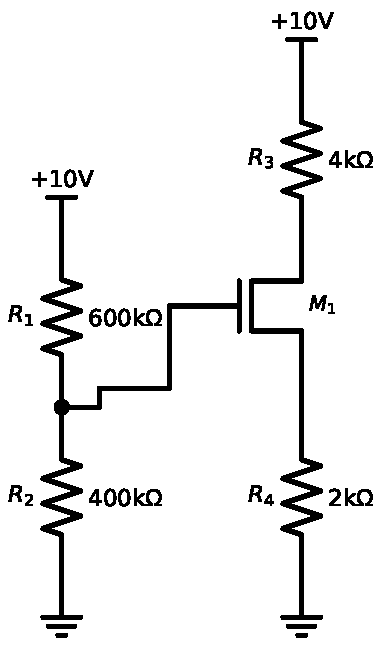
\includegraphics[width=\linewidth,height=7cm,keepaspectratio]{p01_circuit}\end{center}
\end{probbox}

\begin{probbox}{Problem 5A.2 \hfill Easy}
For the circuit below, find the DC drain currents $I_D$ of all transistors and verify their operating modes. Assume $k'_p\frac{W}{L} = 850\,\mu \mathrm{A/V^2}$, $V_{tp} = -1.3$\,V.
\begin{center}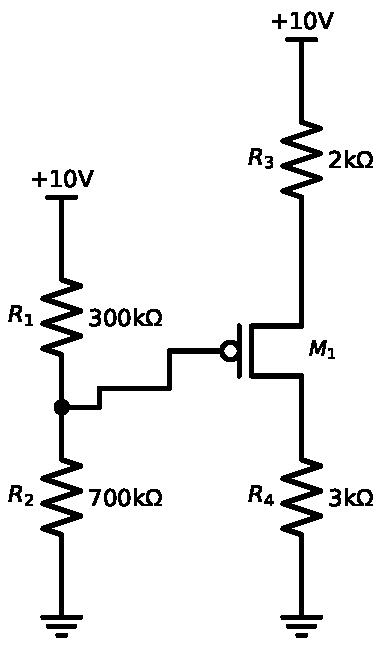
\includegraphics[width=\linewidth,height=7cm,keepaspectratio]{p02_circuit}\end{center}
\end{probbox}

\begin{probbox}{Problem 5A.3 \hfill Easy}
For the circuit below, find the DC drain currents $I_D$ of all transistors and verify their operating modes. Assume $k'_n\frac{W}{L} = 2\,\mathrm{m}\mathrm{A/V^2}$, $V_{tn} = 1$\,V.
\begin{center}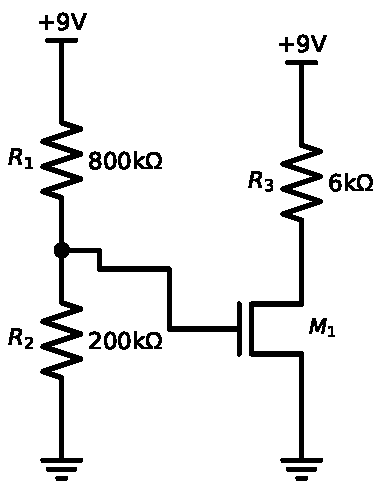
\includegraphics[width=\linewidth,height=7cm,keepaspectratio]{p03_circuit}\end{center}
\end{probbox}

\begin{probbox}{Problem 5A.4 \hfill Easy}
For the circuit below, find the DC drain currents $I_D$ of all transistors and verify their operating modes. Assume $k'_n\frac{W}{L} = 1.1\,\mathrm{m}\mathrm{A/V^2}$, $V_{tn} = 1.4$\,V.
\begin{center}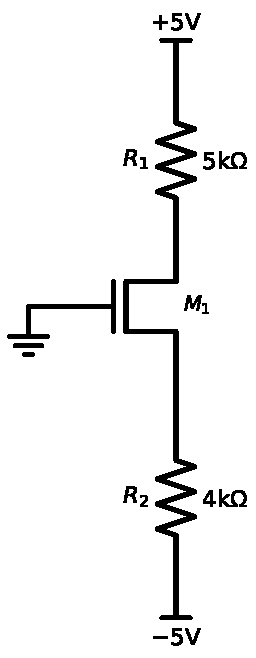
\includegraphics[width=\linewidth,height=7cm,keepaspectratio]{p04_circuit}\end{center}
\end{probbox}

\begin{probbox}{Problem 5A.5 \hfill Easy}
For the circuit below, find the DC drain currents $I_D$ of all transistors and verify their operating modes. Assume $k'_p\frac{W}{L} = 1\,\mathrm{m}\mathrm{A/V^2}$, $V_{tp} = -1$\,V.
\begin{center}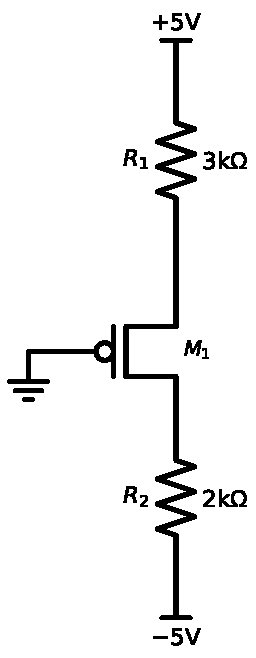
\includegraphics[width=\linewidth,height=7cm,keepaspectratio]{p05_circuit}\end{center}
\end{probbox}

\begin{probbox}{Problem 5A.6 \hfill Easy}
For the circuit below, find the DC drain currents $I_D$ of all transistors and verify their operating modes. Assume $k'_n\frac{W}{L} = 1.1\,\mathrm{m}\mathrm{A/V^2}$, $V_{tn} = 1.4$\,V.
\begin{center}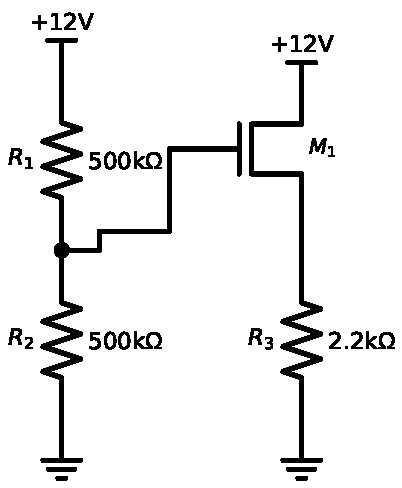
\includegraphics[width=\linewidth,height=7cm,keepaspectratio]{p06_circuit}\end{center}
\end{probbox}

\subsection*{Medium problems}
\begin{probbox}{Problem 5A.7 \hfill Medium}
For the circuit below, find the DC drain currents $I_D$ of all transistors and verify their operating modes. Assume $k'_n\frac{W}{L} = 1.1\,\mathrm{m}\mathrm{A/V^2}$, $V_{tn} = 1.4$\,V, $k'_p\frac{W}{L} = 850\,\mu \mathrm{A/V^2}$, $V_{tp} = -1.3$\,V.
\begin{center}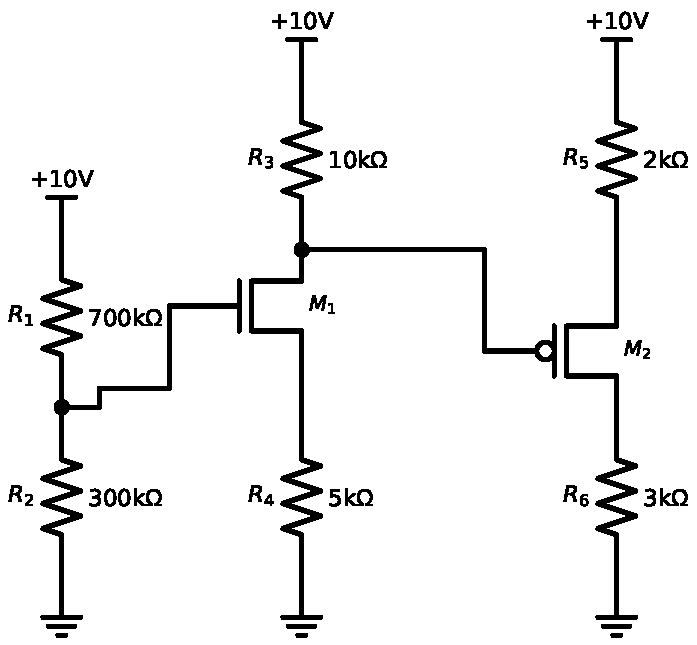
\includegraphics[width=\linewidth,height=7cm,keepaspectratio]{p07_circuit}\end{center}
\end{probbox}

\begin{probbox}{Problem 5A.8 \hfill Medium}
For the circuit below, find the DC drain currents $I_D$ of all transistors and verify their operating modes. Assume $k'_n\frac{W}{L} = 2\,\mathrm{m}\mathrm{A/V^2}$, $V_{tn} = 1$\,V.
\begin{center}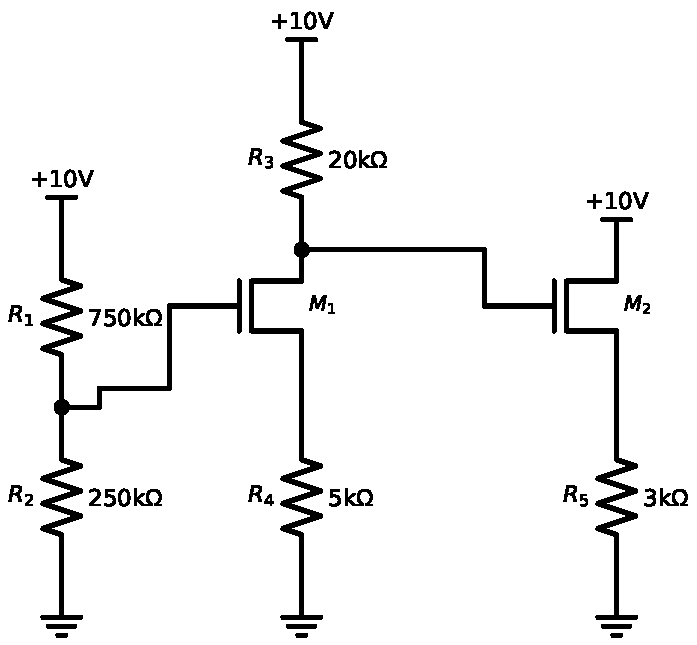
\includegraphics[width=\linewidth,height=7cm,keepaspectratio]{p08_circuit}\end{center}
\end{probbox}

\begin{probbox}{Problem 5A.9 \hfill Medium}
For the circuit below, find the DC drain currents $I_D$ of all transistors and verify their operating modes. Assume $k'_n\frac{W}{L} = 1.1\,\mathrm{m}\mathrm{A/V^2}$, $V_{tn} = 1.4$\,V, $k'_p\frac{W}{L} = 850\,\mu \mathrm{A/V^2}$, $V_{tp} = -1.3$\,V.
\begin{center}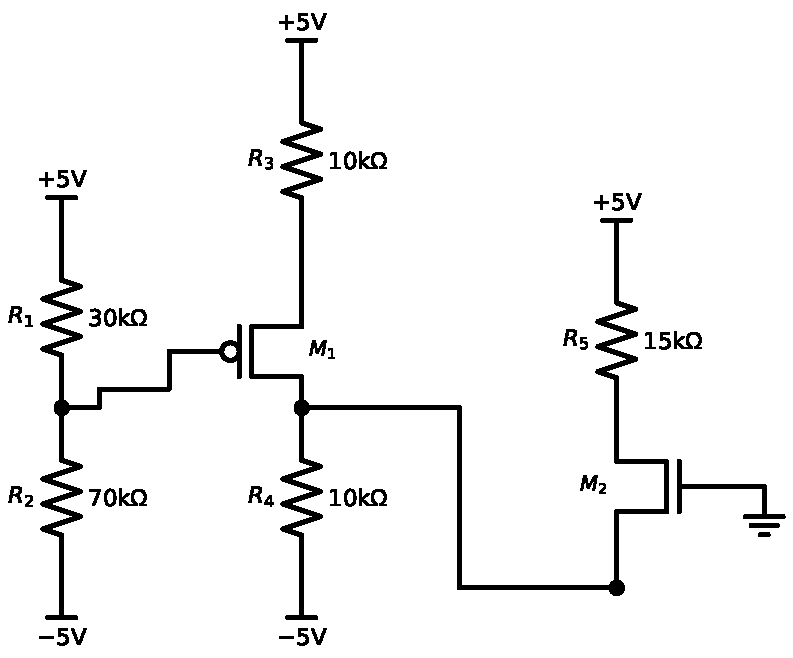
\includegraphics[width=\linewidth,height=7cm,keepaspectratio]{p09_circuit}\end{center}
\end{probbox}

\begin{probbox}{Problem 5A.10 \hfill Medium}
For the circuit below, find the DC drain currents $I_D$ of all transistors and verify their operating modes. Assume $k'_n\frac{W}{L} = 500\,\mu \mathrm{A/V^2}$, $V_{tn} = 0.8$\,V, $k'_p\frac{W}{L} = 400\,\mu \mathrm{A/V^2}$, $V_{tp} = -0.8$\,V.
\begin{center}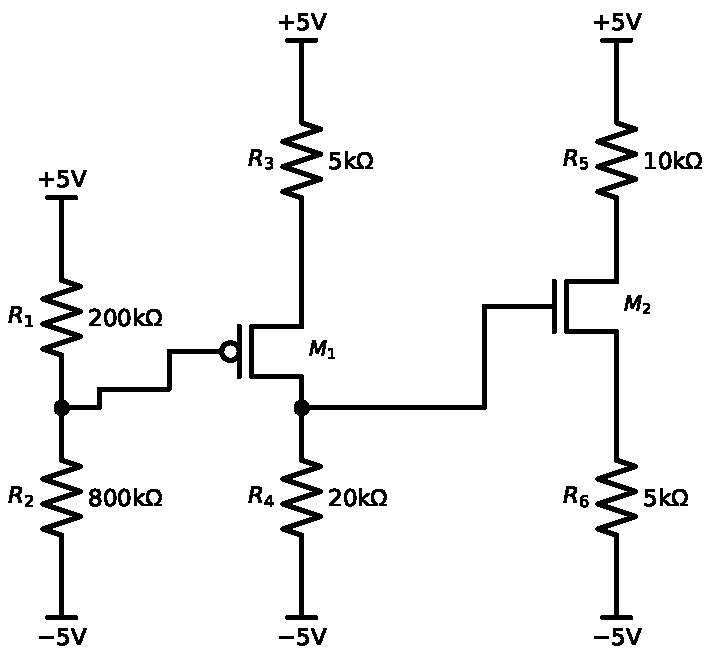
\includegraphics[width=\linewidth,height=7cm,keepaspectratio]{p10_circuit}\end{center}
\end{probbox}

\begin{probbox}{Problem 5A.11 \hfill Medium}
For the circuit below, find the DC drain currents $I_D$ of all transistors and verify their operating modes. Assume $k'_n\frac{W}{L} = 1.1\,\mathrm{m}\mathrm{A/V^2}$, $V_{tn} = 1.4$\,V.
\begin{center}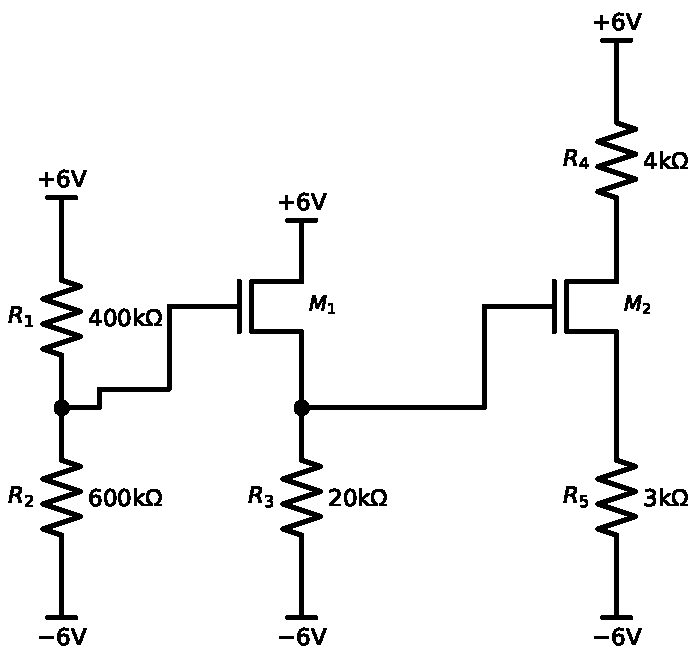
\includegraphics[width=\linewidth,height=7cm,keepaspectratio]{p11_circuit}\end{center}
\end{probbox}

\begin{probbox}{Problem 5A.12 \hfill Medium}
For the circuit below, find the DC drain currents $I_D$ of all transistors and verify their operating modes. Assume $k'_n\frac{W}{L} = 2\,\mathrm{m}\mathrm{A/V^2}$, $V_{tn} = 1$\,V, $k'_p\frac{W}{L} = 1\,\mathrm{m}\mathrm{A/V^2}$, $V_{tp} = -1$\,V.
\begin{center}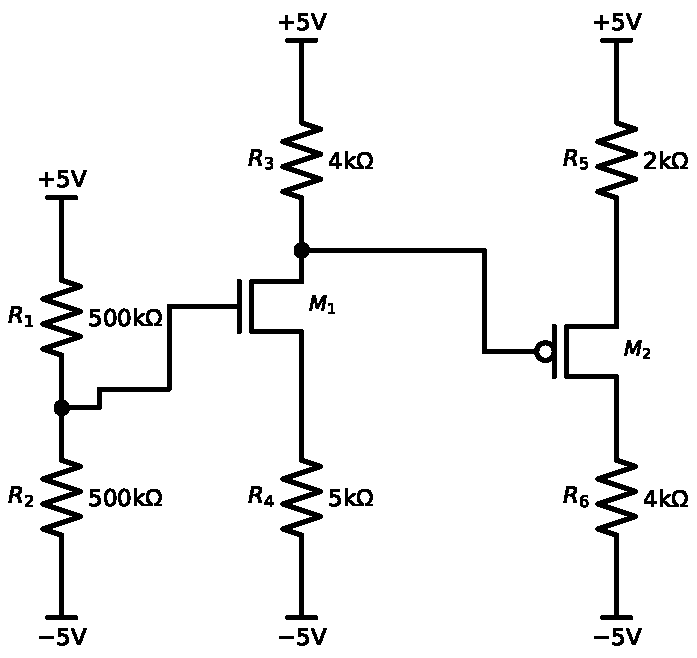
\includegraphics[width=\linewidth,height=7cm,keepaspectratio]{p12_circuit}\end{center}
\end{probbox}

\subsection*{Hard problems}
\begin{probbox}{Problem 5A.13 \hfill Hard}
For the circuit below, find the DC drain currents $I_D$ of all transistors and verify their operating modes. Assume $k'_n\frac{W}{L} = 1.1\,\mathrm{m}\mathrm{A/V^2}$, $V_{tn} = 1.4$\,V, $k'_p\frac{W}{L} = 850\,\mu \mathrm{A/V^2}$, $V_{tp} = -1.3$\,V. (This is Sample Problem 1 of the lecture.)
\begin{center}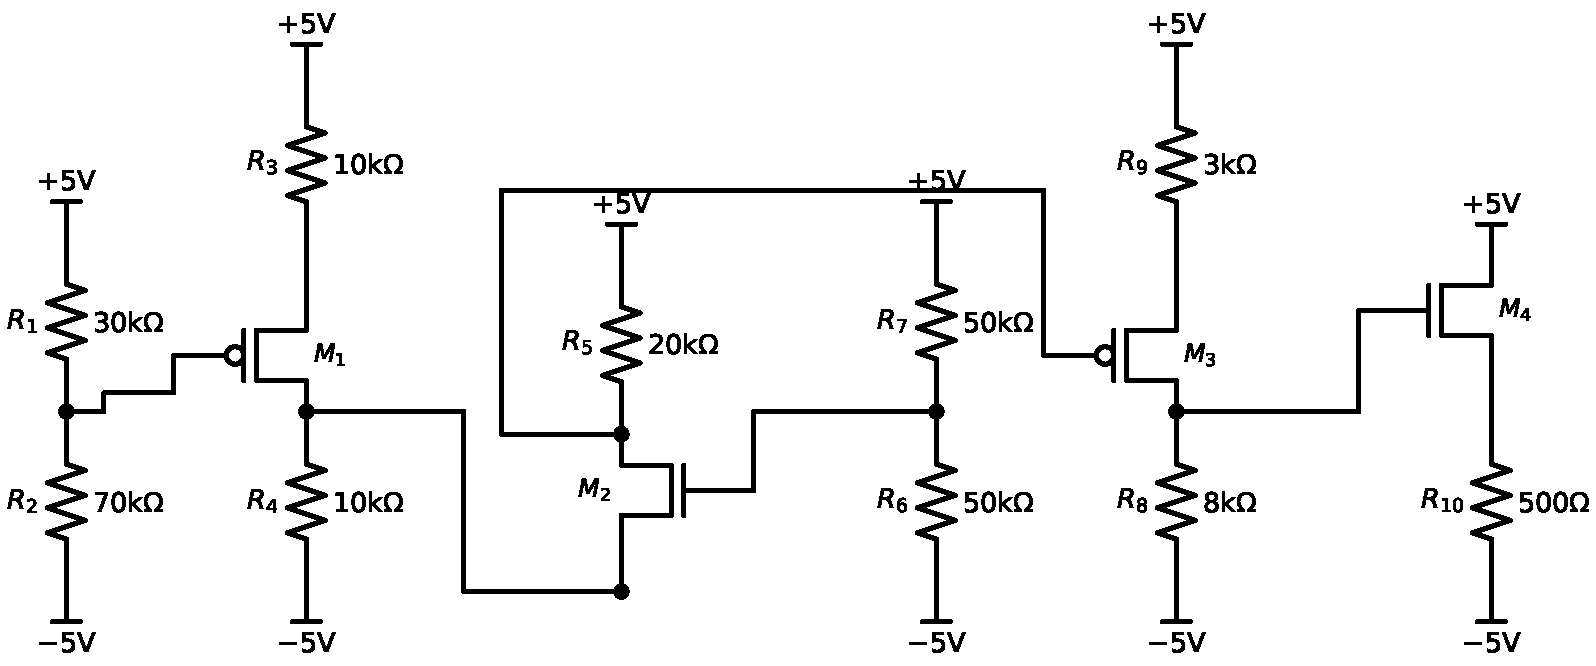
\includegraphics[width=\linewidth,height=7cm,keepaspectratio]{p13_circuit}\end{center}
\end{probbox}

\begin{probbox}{Problem 5A.14 \hfill Hard}
For the circuit below, find the DC drain currents $I_D$ of all transistors and verify their operating modes. Assume $k'_n\frac{W}{L} = 1.1\,\mathrm{m}\mathrm{A/V^2}$, $V_{tn} = 1.4$\,V, $k'_p\frac{W}{L} = 850\,\mu \mathrm{A/V^2}$, $V_{tp} = -1.3$\,V.
\begin{center}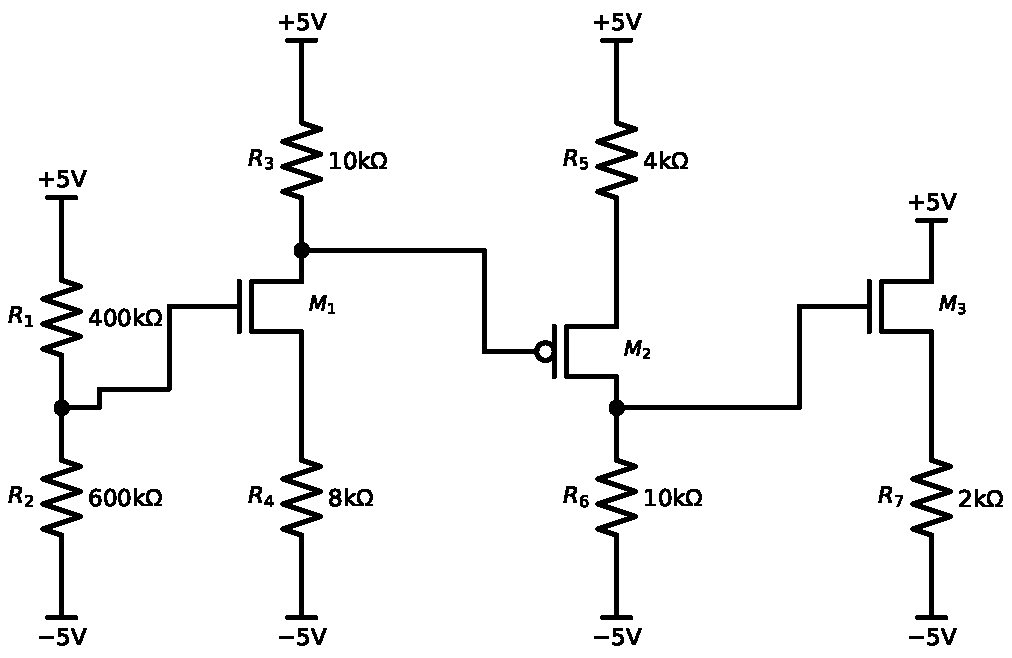
\includegraphics[width=\linewidth,height=7cm,keepaspectratio]{p14_circuit}\end{center}
\end{probbox}

\begin{probbox}{Problem 5A.15 \hfill Hard}
For the circuit below, find the DC drain currents $I_D$ of all transistors and verify their operating modes. Assume $k'_n\frac{W}{L} = 2\,\mathrm{m}\mathrm{A/V^2}$, $V_{tn} = 1$\,V, $k'_p\frac{W}{L} = 1\,\mathrm{m}\mathrm{A/V^2}$, $V_{tp} = -1$\,V.
\begin{center}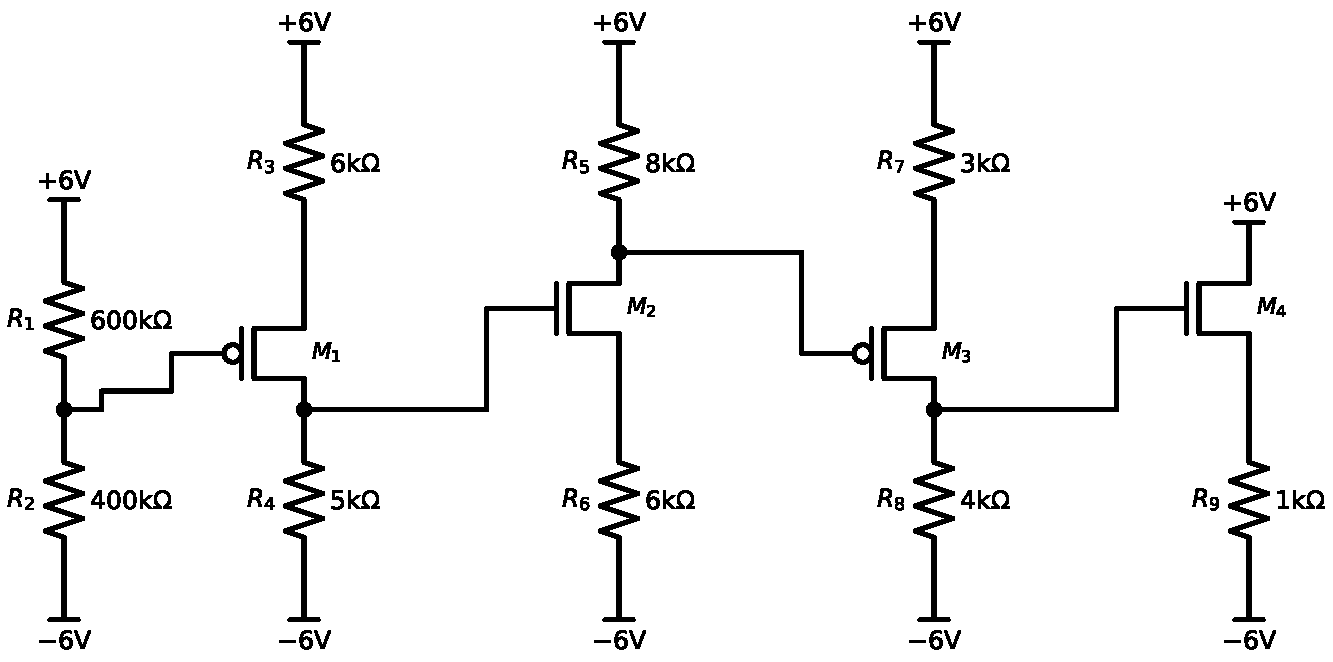
\includegraphics[width=\linewidth,height=7cm,keepaspectratio]{p15_circuit}\end{center}
\end{probbox}

\begin{probbox}{Problem 5A.16 \hfill Hard}
For the circuit below, find the DC drain currents $I_D$ of all transistors and verify their operating modes. Assume $k'_n\frac{W}{L} = 1.1\,\mathrm{m}\mathrm{A/V^2}$, $V_{tn} = 1.4$\,V, $k'_p\frac{W}{L} = 850\,\mu \mathrm{A/V^2}$, $V_{tp} = -1.3$\,V.
\begin{center}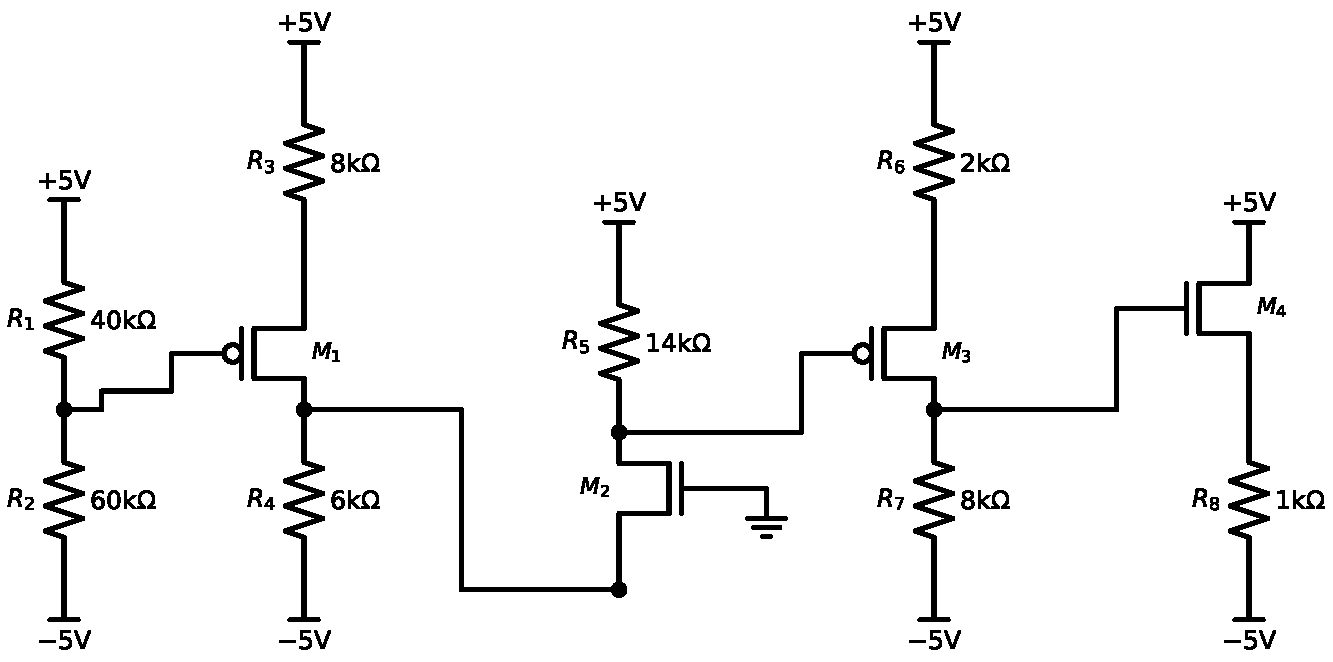
\includegraphics[width=\linewidth,height=7cm,keepaspectratio]{p16_circuit}\end{center}
\end{probbox}

\begin{probbox}{Problem 5A.17 \hfill Hard}
For the circuit below, find the DC drain currents $I_D$ of all transistors and verify their operating modes. Assume $k'_n\frac{W}{L} = 500\,\mu \mathrm{A/V^2}$, $V_{tn} = 0.8$\,V, $k'_p\frac{W}{L} = 400\,\mu \mathrm{A/V^2}$, $V_{tp} = -0.8$\,V.
\begin{center}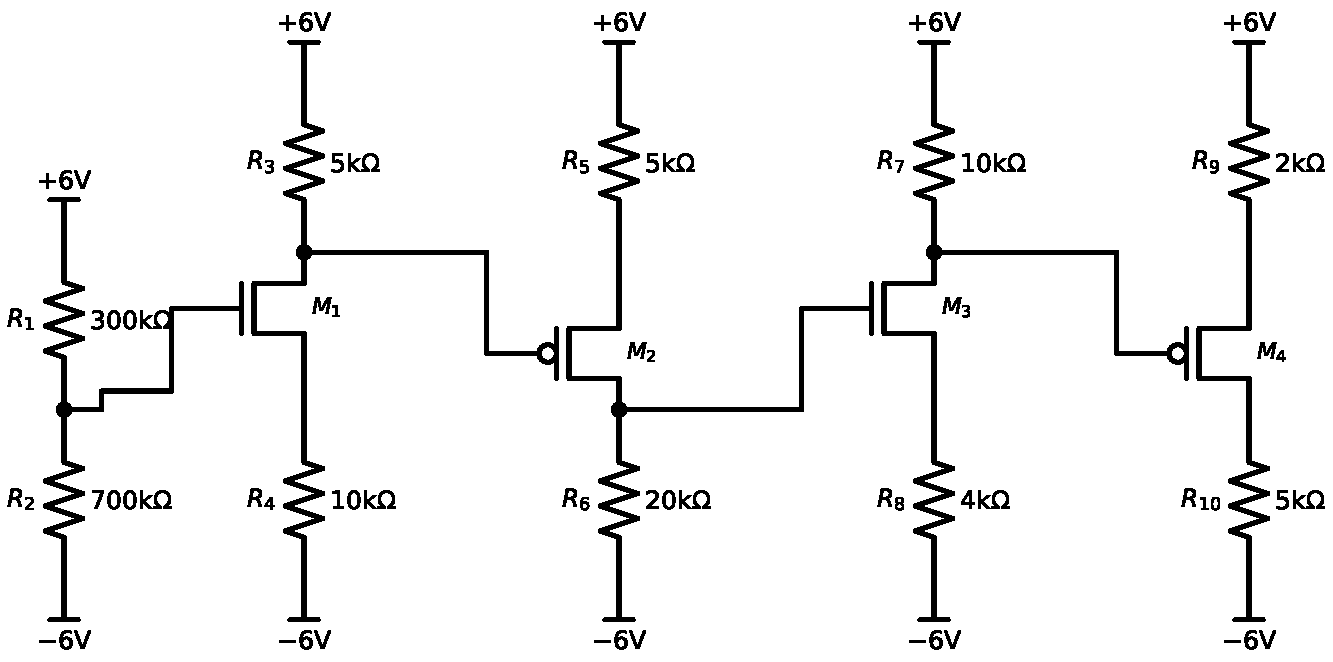
\includegraphics[width=\linewidth,height=7cm,keepaspectratio]{p17_circuit}\end{center}
\end{probbox}

\begin{probbox}{Problem 5A.18 \hfill Hard}
For the circuit below, find the DC drain currents $I_D$ of all transistors and verify their operating modes. Assume $k'_n\frac{W}{L} = 1.1\,\mathrm{m}\mathrm{A/V^2}$, $V_{tn} = 1.4$\,V, $k'_p\frac{W}{L} = 850\,\mu \mathrm{A/V^2}$, $V_{tp} = -1.3$\,V.
\begin{center}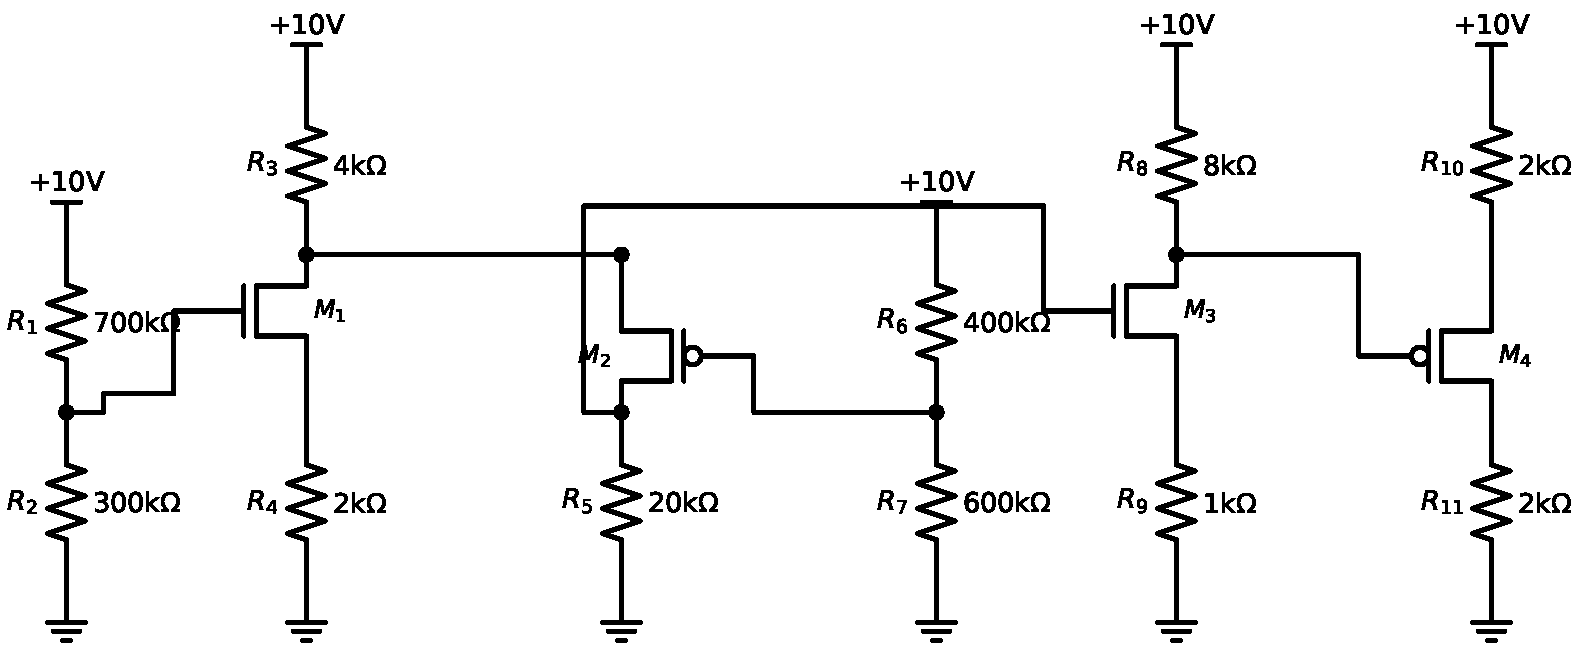
\includegraphics[width=\linewidth,height=7cm,keepaspectratio]{p18_circuit}\end{center}
\end{probbox}

\newpage
\section*{Solutions}
Every solution follows the steps of the Lecture-5 pipeline card.
\subsection*{Solution 5A.1 \hfill Easy}
\begin{center}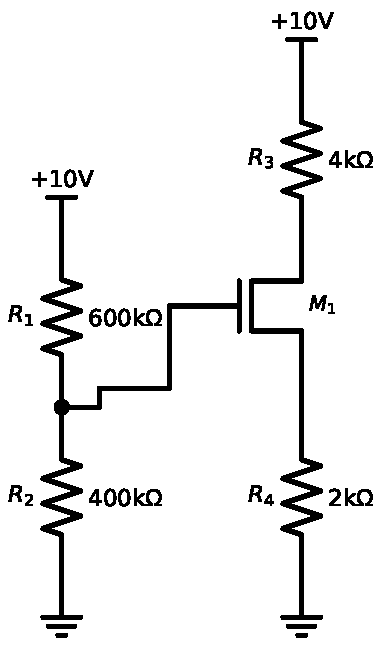
\includegraphics[width=0.9\linewidth,height=6cm,keepaspectratio]{p01_circuit}\end{center}
\solstep{1}{Assumptions}Assume every transistor is active (saturation, tool T1). No current flows into any gate, so gate voltages come from the resistor networks alone.
\solstep{2}{Walk through the circuit}\begin{enumerate}[leftmargin=*,itemsep=3pt]
\item No current flows into a gate ($I_G = 0$), so $V_{G1}$ is set by the divider $R_{1}$--$R_{2}$:\[V_{G1} = 0 + (10 - 0)\frac{400\,\mathrm{k}}{600\,\mathrm{k} + 400\,\mathrm{k}} = 4\,\mathrm{V}\]
\item KVL from the gate of $M_{1}$ through $V_{GS1}$ and $R_{4}$ ($I_G = 0$, $M_{1}$ assumed active):\[V_{G1} - 0 = 4 = V_{GS1} + R_{4}I_{D1}\]\[I_{D1} = \frac{4 - V_{GS1}}{2\,\mathrm{k}} = \frac{1.1\,\mathrm{m}}{2}(V_{GS1} - 1.4)^2\]\[1.1V_{GS1}^2 - 2.08V_{GS1} - 1.844 = 0 \;\Rightarrow\; V_{GS1} = -0.6577\ \text{or}\ 2.549\,\mathrm{V}\]The root $-0.658$\,V is below $|V_t| = 1.4$\,V (the transistor would be off), so $V_{GS1} = 2.549$\,V. Then $I_{D1} = 726\,\mu \mathrm{A}$ and $V_{S1} = V_{G1} - V_{GS1} = 1.45\,\mathrm{V}$.
\item $I_{D1}$ flows from $10$ through $R_{3}$: $V_{D1} = 10 - R_{3}I_{D1} = 10 - 4\,\mathrm{k}\times726\,\mu \mathrm{A} = 7.1\,\mathrm{V}$.
\end{enumerate}

\solstep{3}{Verify the operating modes}\begin{itemize}[leftmargin=*,itemsep=2pt]
\item $V_{DS1} = V_{D1} - V_{S1} = 7.097 - 1.451 = 5.65\,\mathrm{V}$ $\ge V_{ov1} = 1.15$\,V $\Rightarrow$ $M_{1}$ is active \checkmark
\end{itemize}
Unlike the BJT, nothing was neglected here ($I_G = 0$ exactly), so these results are exact for the square-law model: a full nodal solve of the circuit gives the same currents.
\begin{ansbox}
$I_{D1} = 726\,\mu \mathrm{A}$\\[2pt] all transistors active.
\end{ansbox}

\newpage
\subsection*{Solution 5A.2 \hfill Easy}
\begin{center}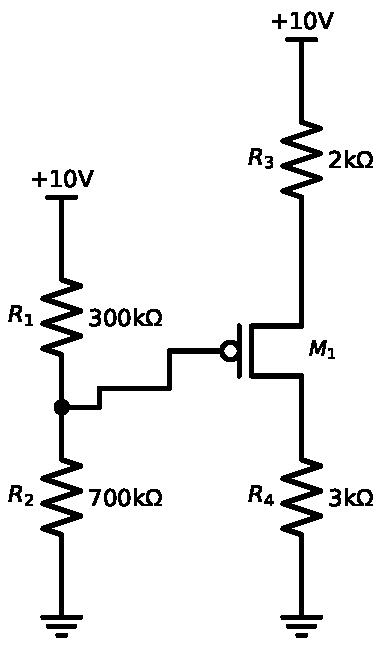
\includegraphics[width=0.9\linewidth,height=6cm,keepaspectratio]{p02_circuit}\end{center}
\solstep{1}{Assumptions}Assume every transistor is active (saturation, tool T1). No current flows into any gate, so gate voltages come from the resistor networks alone.
\solstep{2}{Walk through the circuit}\begin{enumerate}[leftmargin=*,itemsep=3pt]
\item No current flows into a gate ($I_G = 0$), so $V_{G1}$ is set by the divider $R_{1}$--$R_{2}$:\[V_{G1} = 0 + (10 - 0)\frac{700\,\mathrm{k}}{300\,\mathrm{k} + 700\,\mathrm{k}} = 7\,\mathrm{V}\]
\item KVL from the gate of $M_{1}$ through $V_{SG1}$ and $R_{3}$ ($I_G = 0$, $M_{1}$ assumed active):\[10 - V_{G1} = 3 = V_{SG1} + R_{3}I_{D1}\]\[I_{D1} = \frac{3 - V_{SG1}}{2\,\mathrm{k}} = \frac{850\,\mu }{2}(V_{SG1} - 1.3)^2\]\[0.85V_{SG1}^2 - 1.21V_{SG1} - 1.563 = 0 \;\Rightarrow\; V_{SG1} = -0.8199\ \text{or}\ 2.243\,\mathrm{V}\]The root $-0.82$\,V is below $|V_t| = 1.3$\,V (the transistor would be off), so $V_{SG1} = 2.243$\,V. Then $I_{D1} = 378\,\mu \mathrm{A}$ and $V_{S1} = V_{G1} + V_{SG1} = 9.24\,\mathrm{V}$.
\item $I_{D1} = 378\,\mu \mathrm{A}$ flows through $R_{4}$ to $0$: $V_{D1} = 0 + R_{4}I_{D1} = 0 + 3\,\mathrm{k}\times378\,\mu \mathrm{A} = 1.13\,\mathrm{V}$.
\end{enumerate}

\solstep{3}{Verify the operating modes}\begin{itemize}[leftmargin=*,itemsep=2pt]
\item $V_{SD1} = V_{S1} - V_{D1} = 9.243 - 1.135 = 8.11\,\mathrm{V}$ $\ge V_{ov1} = 0.943$\,V $\Rightarrow$ $M_{1}$ is active \checkmark
\end{itemize}
Unlike the BJT, nothing was neglected here ($I_G = 0$ exactly), so these results are exact for the square-law model: a full nodal solve of the circuit gives the same currents.
\begin{ansbox}
$I_{D1} = 378\,\mu \mathrm{A}$\\[2pt] all transistors active.
\end{ansbox}

\newpage
\subsection*{Solution 5A.3 \hfill Easy}
\begin{center}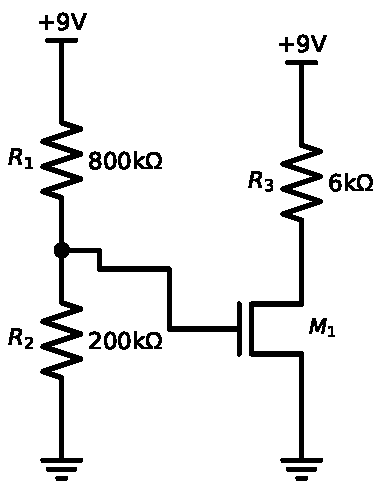
\includegraphics[width=0.9\linewidth,height=6cm,keepaspectratio]{p03_circuit}\end{center}
\solstep{1}{Assumptions}Assume every transistor is active (saturation, tool T1). No current flows into any gate, so gate voltages come from the resistor networks alone.
\solstep{2}{Walk through the circuit}\begin{enumerate}[leftmargin=*,itemsep=3pt]
\item No current flows into a gate ($I_G = 0$), so $V_{G1}$ is set by the divider $R_{1}$--$R_{2}$:\[V_{G1} = 0 + (9 - 0)\frac{200\,\mathrm{k}}{800\,\mathrm{k} + 200\,\mathrm{k}} = 1.8\,\mathrm{V}\]
\item Gate and source of $M_{1}$ are known: $V_{GS1} = 1.8$\,V, $V_{ov1} = 0.8$\,V, so $I_{D1} = \frac{k_{1}}{2}V_{ov1}^2 = 640\,\mu \mathrm{A}$.
\item $I_{D1}$ flows from $9$ through $R_{3}$: $V_{D1} = 9 - R_{3}I_{D1} = 9 - 6\,\mathrm{k}\times640\,\mu \mathrm{A} = 5.16\,\mathrm{V}$.
\end{enumerate}

\solstep{3}{Verify the operating modes}\begin{itemize}[leftmargin=*,itemsep=2pt]
\item $V_{DS1} = V_{D1} - 0 = 5.16 - 0 = 5.16\,\mathrm{V}$ $\ge V_{ov1} = 0.8$\,V $\Rightarrow$ $M_{1}$ is active \checkmark
\end{itemize}
Unlike the BJT, nothing was neglected here ($I_G = 0$ exactly), so these results are exact for the square-law model: a full nodal solve of the circuit gives the same currents.
\begin{ansbox}
$I_{D1} = 640\,\mu \mathrm{A}$\\[2pt] all transistors active.
\end{ansbox}

\newpage
\subsection*{Solution 5A.4 \hfill Easy}
\begin{center}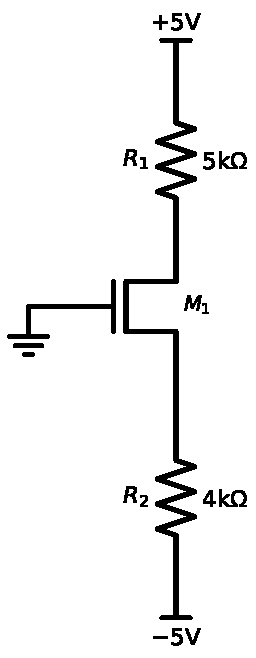
\includegraphics[width=0.9\linewidth,height=6cm,keepaspectratio]{p04_circuit}\end{center}
\solstep{1}{Assumptions}Assume every transistor is active (saturation, tool T1). No current flows into any gate, so gate voltages come from the resistor networks alone.
\solstep{2}{Walk through the circuit}\begin{enumerate}[leftmargin=*,itemsep=3pt]
\item KVL from the gate of $M_{1}$ through $V_{GS1}$ and $R_{2}$ ($I_G = 0$, $M_{1}$ assumed active):\[0 - (-5) = 5 = V_{GS1} + R_{2}I_{D1}\]\[I_{D1} = \frac{5 - V_{GS1}}{4\,\mathrm{k}} = \frac{1.1\,\mathrm{m}}{2}(V_{GS1} - 1.4)^2\]\[2.2V_{GS1}^2 - 5.16V_{GS1} - 0.688 = 0 \;\Rightarrow\; V_{GS1} = -0.1265\ \text{or}\ 2.472\,\mathrm{V}\]The root $-0.127$\,V is below $|V_t| = 1.4$\,V (the transistor would be off), so $V_{GS1} = 2.472$\,V. Then $I_{D1} = 632\,\mu \mathrm{A}$ and $V_{S1} = 0 - V_{GS1} = -2.47\,\mathrm{V}$.
\item $I_{D1}$ flows from $5$ through $R_{1}$: $V_{D1} = 5 - R_{1}I_{D1} = 5 - 5\,\mathrm{k}\times632\,\mu \mathrm{A} = 1.84\,\mathrm{V}$.
\end{enumerate}

\solstep{3}{Verify the operating modes}\begin{itemize}[leftmargin=*,itemsep=2pt]
\item $V_{DS1} = V_{D1} - V_{S1} = 1.84 - (-2.472) = 4.31\,\mathrm{V}$ $\ge V_{ov1} = 1.07$\,V $\Rightarrow$ $M_{1}$ is active \checkmark
\end{itemize}
Unlike the BJT, nothing was neglected here ($I_G = 0$ exactly), so these results are exact for the square-law model: a full nodal solve of the circuit gives the same currents.
\begin{ansbox}
$I_{D1} = 632\,\mu \mathrm{A}$\\[2pt] all transistors active.
\end{ansbox}

\newpage
\subsection*{Solution 5A.5 \hfill Easy}
\begin{center}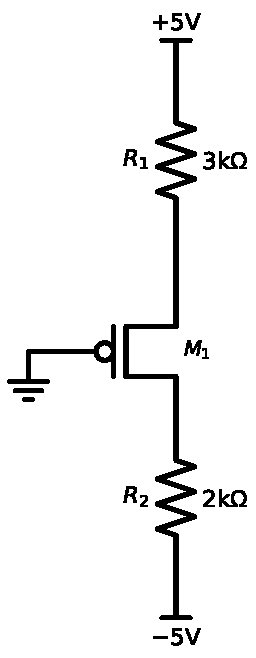
\includegraphics[width=0.9\linewidth,height=6cm,keepaspectratio]{p05_circuit}\end{center}
\solstep{1}{Assumptions}Assume every transistor is active (saturation, tool T1). No current flows into any gate, so gate voltages come from the resistor networks alone.
\solstep{2}{Walk through the circuit}\begin{enumerate}[leftmargin=*,itemsep=3pt]
\item KVL from the gate of $M_{1}$ through $V_{SG1}$ and $R_{1}$ ($I_G = 0$, $M_{1}$ assumed active):\[5 - 0 = 5 = V_{SG1} + R_{1}I_{D1}\]\[I_{D1} = \frac{5 - V_{SG1}}{3\,\mathrm{k}} = \frac{1\,\mathrm{m}}{2}(V_{SG1} - 1)^2\]\[1.5V_{SG1}^2 - 2V_{SG1} - 3.5 = 0 \;\Rightarrow\; V_{SG1} = -1\ \text{or}\ 2.333\,\mathrm{V}\]The root $-1$\,V is below $|V_t| = 1$\,V (the transistor would be off), so $V_{SG1} = 2.333$\,V. Then $I_{D1} = 889\,\mu \mathrm{A}$ and $V_{S1} = 0 + V_{SG1} = 2.33\,\mathrm{V}$.
\item $I_{D1} = 889\,\mu \mathrm{A}$ flows through $R_{2}$ to $(-5)$: $V_{D1} = (-5) + R_{2}I_{D1} = -5 + 2\,\mathrm{k}\times889\,\mu \mathrm{A} = -3.22\,\mathrm{V}$.
\end{enumerate}

\solstep{3}{Verify the operating modes}\begin{itemize}[leftmargin=*,itemsep=2pt]
\item $V_{SD1} = V_{S1} - V_{D1} = 2.333 - (-3.222) = 5.56\,\mathrm{V}$ $\ge V_{ov1} = 1.33$\,V $\Rightarrow$ $M_{1}$ is active \checkmark
\end{itemize}
Unlike the BJT, nothing was neglected here ($I_G = 0$ exactly), so these results are exact for the square-law model: a full nodal solve of the circuit gives the same currents.
\begin{ansbox}
$I_{D1} = 889\,\mu \mathrm{A}$\\[2pt] all transistors active.
\end{ansbox}

\newpage
\subsection*{Solution 5A.6 \hfill Easy}
\begin{center}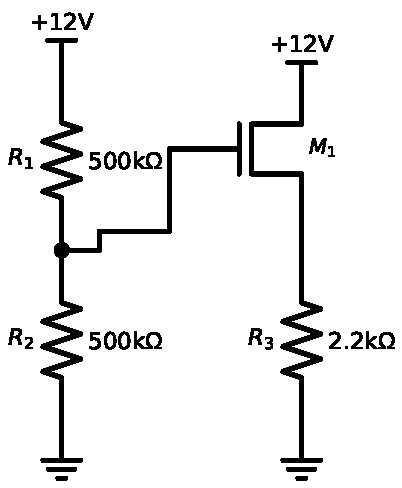
\includegraphics[width=0.9\linewidth,height=6cm,keepaspectratio]{p06_circuit}\end{center}
\solstep{1}{Assumptions}Assume every transistor is active (saturation, tool T1). No current flows into any gate, so gate voltages come from the resistor networks alone.
\solstep{2}{Walk through the circuit}\begin{enumerate}[leftmargin=*,itemsep=3pt]
\item No current flows into a gate ($I_G = 0$), so $V_{G1}$ is set by the divider $R_{1}$--$R_{2}$:\[V_{G1} = 0 + (12 - 0)\frac{500\,\mathrm{k}}{500\,\mathrm{k} + 500\,\mathrm{k}} = 6\,\mathrm{V}\]
\item KVL from the gate of $M_{1}$ through $V_{GS1}$ and $R_{3}$ ($I_G = 0$, $M_{1}$ assumed active):\[V_{G1} - 0 = 6 = V_{GS1} + R_{3}I_{D1}\]\[I_{D1} = \frac{6 - V_{GS1}}{2.2\,\mathrm{k}} = \frac{1.1\,\mathrm{m}}{2}(V_{GS1} - 1.4)^2\]\[1.21V_{GS1}^2 - 2.388V_{GS1} - 3.628 = 0 \;\Rightarrow\; V_{GS1} = -1.006\ \text{or}\ 2.98\,\mathrm{V}\]The root $-1.01$\,V is below $|V_t| = 1.4$\,V (the transistor would be off), so $V_{GS1} = 2.98$\,V. Then $I_{D1} = 1.37\,\mathrm{m}\mathrm{A}$ and $V_{S1} = V_{G1} - V_{GS1} = 3.02\,\mathrm{V}$.
\end{enumerate}

\solstep{3}{Verify the operating modes}\begin{itemize}[leftmargin=*,itemsep=2pt]
\item $V_{DS1} = 12 - V_{S1} = 12 - 3.02 = 8.98\,\mathrm{V}$ $\ge V_{ov1} = 1.58$\,V $\Rightarrow$ $M_{1}$ is active \checkmark
\end{itemize}
Unlike the BJT, nothing was neglected here ($I_G = 0$ exactly), so these results are exact for the square-law model: a full nodal solve of the circuit gives the same currents.
\begin{ansbox}
$I_{D1} = 1.37\,\mathrm{m}\mathrm{A}$\\[2pt] all transistors active.
\end{ansbox}

\newpage
\subsection*{Solution 5A.7 \hfill Medium}
\begin{center}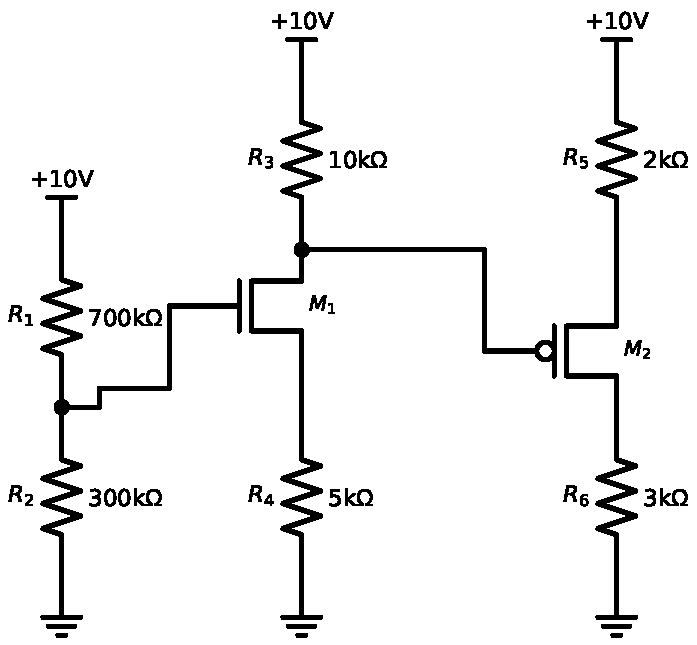
\includegraphics[width=0.9\linewidth,height=6cm,keepaspectratio]{p07_circuit}\end{center}
\solstep{1}{Assumptions}Assume every transistor is active (saturation, tool T1). No current flows into any gate, so gate voltages come from the resistor networks alone.
\solstep{2}{Walk through the circuit}\begin{enumerate}[leftmargin=*,itemsep=3pt]
\item No current flows into a gate ($I_G = 0$), so $V_{G1}$ is set by the divider $R_{1}$--$R_{2}$:\[V_{G1} = 0 + (10 - 0)\frac{300\,\mathrm{k}}{700\,\mathrm{k} + 300\,\mathrm{k}} = 3\,\mathrm{V}\]
\item KVL from the gate of $M_{1}$ through $V_{GS1}$ and $R_{4}$ ($I_G = 0$, $M_{1}$ assumed active):\[V_{G1} - 0 = 3 = V_{GS1} + R_{4}I_{D1}\]\[I_{D1} = \frac{3 - V_{GS1}}{5\,\mathrm{k}} = \frac{1.1\,\mathrm{m}}{2}(V_{GS1} - 1.4)^2\]\[2.75V_{GS1}^2 - 6.7V_{GS1} + 2.39 = 0 \;\Rightarrow\; V_{GS1} = 0.434\ \text{or}\ 2.002\,\mathrm{V}\]The root $0.434$\,V is below $|V_t| = 1.4$\,V (the transistor would be off), so $V_{GS1} = 2.002$\,V. Then $I_{D1} = 200\,\mu \mathrm{A}$ and $V_{S1} = V_{G1} - V_{GS1} = 0.998\,\mathrm{V}$.
\item $I_{D1}$ flows from $10$ through $R_{3}$: $V_{D1} = 10 - R_{3}I_{D1} = 10 - 10\,\mathrm{k}\times200\,\mu \mathrm{A} = 8\,\mathrm{V}$.
\item KVL from the gate of $M_{2}$ through $V_{SG2}$ and $R_{5}$ ($I_G = 0$, $M_{2}$ assumed active):\[10 - V_{D1} = 1.995 = V_{SG2} + R_{5}I_{D2}\]\[I_{D2} = \frac{1.995 - V_{SG2}}{2\,\mathrm{k}} = \frac{850\,\mu }{2}(V_{SG2} - 1.3)^2\]\[0.85V_{SG2}^2 - 1.21V_{SG2} - 0.5589 = 0 \;\Rightarrow\; V_{SG2} = -0.3672\ \text{or}\ 1.791\,\mathrm{V}\]The root $-0.367$\,V is below $|V_t| = 1.3$\,V (the transistor would be off), so $V_{SG2} = 1.791$\,V. Then $I_{D2} = 102\,\mu \mathrm{A}$ and $V_{S2} = V_{D1} + V_{SG2} = 9.8\,\mathrm{V}$.
\item $I_{D2} = 102\,\mu \mathrm{A}$ flows through $R_{6}$ to $0$: $V_{D2} = 0 + R_{6}I_{D2} = 0 + 3\,\mathrm{k}\times102\,\mu \mathrm{A} = 0.307\,\mathrm{V}$.
\end{enumerate}

\solstep{3}{Verify the operating modes}\begin{itemize}[leftmargin=*,itemsep=2pt]
\item $V_{DS1} = V_{D1} - V_{S1} = 8.005 - 0.9977 = 7.01\,\mathrm{V}$ $\ge V_{ov1} = 0.602$\,V $\Rightarrow$ $M_{1}$ is active \checkmark
\item $V_{SD2} = V_{S2} - V_{D2} = 9.795 - 0.307 = 9.49\,\mathrm{V}$ $\ge V_{ov2} = 0.491$\,V $\Rightarrow$ $M_{2}$ is active \checkmark
\end{itemize}
Unlike the BJT, nothing was neglected here ($I_G = 0$ exactly), so these results are exact for the square-law model: a full nodal solve of the circuit gives the same currents.
\begin{ansbox}
$I_{D1} = 200\,\mu \mathrm{A}$,\quad $I_{D2} = 102\,\mu \mathrm{A}$\\[2pt] all transistors active.
\end{ansbox}

\newpage
\subsection*{Solution 5A.8 \hfill Medium}
\begin{center}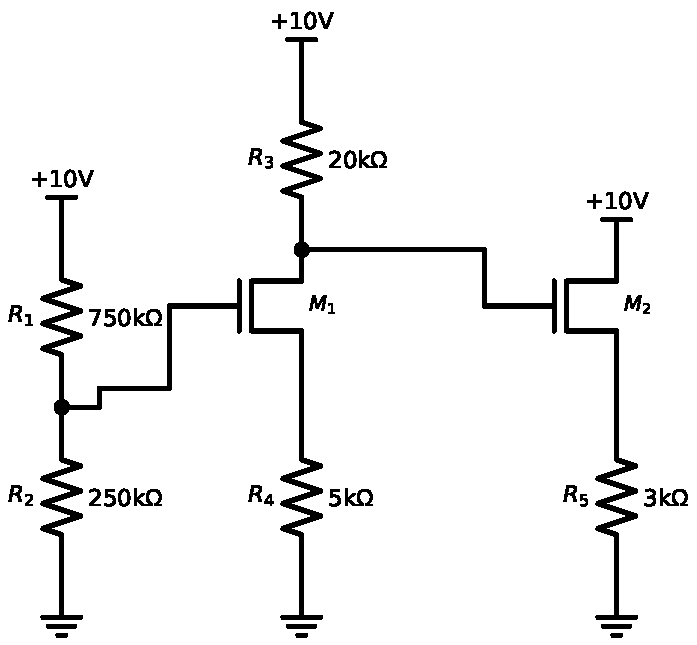
\includegraphics[width=0.9\linewidth,height=6cm,keepaspectratio]{p08_circuit}\end{center}
\solstep{1}{Assumptions}Assume every transistor is active (saturation, tool T1). No current flows into any gate, so gate voltages come from the resistor networks alone.
\solstep{2}{Walk through the circuit}\begin{enumerate}[leftmargin=*,itemsep=3pt]
\item No current flows into a gate ($I_G = 0$), so $V_{G1}$ is set by the divider $R_{1}$--$R_{2}$:\[V_{G1} = 0 + (10 - 0)\frac{250\,\mathrm{k}}{750\,\mathrm{k} + 250\,\mathrm{k}} = 2.5\,\mathrm{V}\]
\item KVL from the gate of $M_{1}$ through $V_{GS1}$ and $R_{4}$ ($I_G = 0$, $M_{1}$ assumed active):\[V_{G1} - 0 = 2.5 = V_{GS1} + R_{4}I_{D1}\]\[I_{D1} = \frac{2.5 - V_{GS1}}{5\,\mathrm{k}} = \frac{2\,\mathrm{m}}{2}(V_{GS1} - 1)^2\]\[5V_{GS1}^2 - 9V_{GS1} + 2.5 = 0 \;\Rightarrow\; V_{GS1} = 0.3432\ \text{or}\ 1.457\,\mathrm{V}\]The root $0.343$\,V is below $|V_t| = 1$\,V (the transistor would be off), so $V_{GS1} = 1.457$\,V. Then $I_{D1} = 209\,\mu \mathrm{A}$ and $V_{S1} = V_{G1} - V_{GS1} = 1.04\,\mathrm{V}$.
\item $I_{D1}$ flows from $10$ through $R_{3}$: $V_{D1} = 10 - R_{3}I_{D1} = 10 - 20\,\mathrm{k}\times209\,\mu \mathrm{A} = 5.83\,\mathrm{V}$.
\item KVL from the gate of $M_{2}$ through $V_{GS2}$ and $R_{5}$ ($I_G = 0$, $M_{2}$ assumed active):\[V_{D1} - 0 = 5.827 = V_{GS2} + R_{5}I_{D2}\]\[I_{D2} = \frac{5.827 - V_{GS2}}{3\,\mathrm{k}} = \frac{2\,\mathrm{m}}{2}(V_{GS2} - 1)^2\]\[3V_{GS2}^2 - 5V_{GS2} - 2.827 = 0 \;\Rightarrow\; V_{GS2} = -0.446\ \text{or}\ 2.113\,\mathrm{V}\]The root $-0.446$\,V is below $|V_t| = 1$\,V (the transistor would be off), so $V_{GS2} = 2.113$\,V. Then $I_{D2} = 1.24\,\mathrm{m}\mathrm{A}$ and $V_{S2} = V_{D1} - V_{GS2} = 3.71\,\mathrm{V}$.
\end{enumerate}

\solstep{3}{Verify the operating modes}\begin{itemize}[leftmargin=*,itemsep=2pt]
\item $V_{DS1} = V_{D1} - V_{S1} = 5.827 - 1.043 = 4.78\,\mathrm{V}$ $\ge V_{ov1} = 0.457$\,V $\Rightarrow$ $M_{1}$ is active \checkmark
\item $V_{DS2} = 10 - V_{S2} = 10 - 3.714 = 6.29\,\mathrm{V}$ $\ge V_{ov2} = 1.11$\,V $\Rightarrow$ $M_{2}$ is active \checkmark
\end{itemize}
Unlike the BJT, nothing was neglected here ($I_G = 0$ exactly), so these results are exact for the square-law model: a full nodal solve of the circuit gives the same currents.
\begin{ansbox}
$I_{D1} = 209\,\mu \mathrm{A}$,\quad $I_{D2} = 1.24\,\mathrm{m}\mathrm{A}$\\[2pt] all transistors active.
\end{ansbox}

\newpage
\subsection*{Solution 5A.9 \hfill Medium}
\begin{center}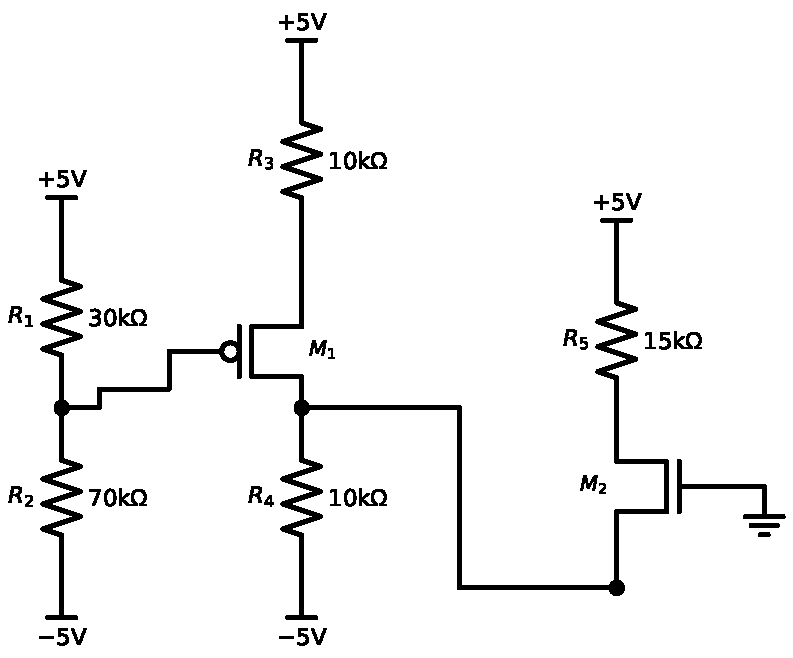
\includegraphics[width=0.9\linewidth,height=6cm,keepaspectratio]{p09_circuit}\end{center}
\solstep{1}{Assumptions}Assume every transistor is active (saturation, tool T1). No current flows into any gate, so gate voltages come from the resistor networks alone.
\solstep{2}{Walk through the circuit}\begin{enumerate}[leftmargin=*,itemsep=3pt]
\item No current flows into a gate ($I_G = 0$), so $V_{G1}$ is set by the divider $R_{1}$--$R_{2}$:\[V_{G1} = -5 + (5 - (-5))\frac{70\,\mathrm{k}}{30\,\mathrm{k} + 70\,\mathrm{k}} = 2\,\mathrm{V}\]
\item KVL from the gate of $M_{1}$ through $V_{SG1}$ and $R_{3}$ ($I_G = 0$, $M_{1}$ assumed active):\[5 - V_{G1} = 3 = V_{SG1} + R_{3}I_{D1}\]\[I_{D1} = \frac{3 - V_{SG1}}{10\,\mathrm{k}} = \frac{850\,\mu }{2}(V_{SG1} - 1.3)^2\]\[4.25V_{SG1}^2 - 10.05V_{SG1} + 4.183 = 0 \;\Rightarrow\; V_{SG1} = 0.539\ \text{or}\ 1.826\,\mathrm{V}\]The root $0.539$\,V is below $|V_t| = 1.3$\,V (the transistor would be off), so $V_{SG1} = 1.826$\,V. Then $I_{D1} = 117\,\mu \mathrm{A}$ and $V_{S1} = V_{G1} + V_{SG1} = 3.83\,\mathrm{V}$.
\item KVL from the gate of $M_{2}$ through $V_{GS2}$ and $R_{4}$ ($I_G = 0$, $M_{2}$ assumed active):\[0 - (-5) = 5 = V_{GS2} + R_{4}(I_{D2} + I_{D1})\]\[I_{D2} = \frac{5 - 10\,\mathrm{k}\times117\,\mu \mathrm{A} - V_{GS2}}{10\,\mathrm{k}} = \frac{1.1\,\mathrm{m}}{2}(V_{GS2} - 1.4)^2\]\[5.5V_{GS2}^2 - 14.4V_{GS2} + 6.954 = 0 \;\Rightarrow\; V_{GS2} = 0.6388\ \text{or}\ 1.979\,\mathrm{V}\]The root $0.639$\,V is below $|V_t| = 1.4$\,V (the transistor would be off), so $V_{GS2} = 1.979$\,V. Then $I_{D2} = 185\,\mu \mathrm{A}$ and $V_{D1} = 0 - V_{GS2} = -1.98\,\mathrm{V}$.
\item $I_{D2}$ flows from $5$ through $R_{5}$: $V_{D2} = 5 - R_{5}I_{D2} = 5 - 15\,\mathrm{k}\times185\,\mu \mathrm{A} = 2.23\,\mathrm{V}$.
\end{enumerate}

\solstep{3}{Verify the operating modes}\begin{itemize}[leftmargin=*,itemsep=2pt]
\item $V_{SD1} = V_{S1} - V_{D1} = 3.826 - (-1.979) = 5.81\,\mathrm{V}$ $\ge V_{ov1} = 0.526$\,V $\Rightarrow$ $M_{1}$ is active \checkmark
\item $V_{DS2} = V_{D2} - V_{D1} = 2.231 - (-1.979) = 4.21\,\mathrm{V}$ $\ge V_{ov2} = 0.579$\,V $\Rightarrow$ $M_{2}$ is active \checkmark
\end{itemize}
Unlike the BJT, nothing was neglected here ($I_G = 0$ exactly), so these results are exact for the square-law model: a full nodal solve of the circuit gives the same currents.
\begin{ansbox}
$I_{D1} = 117\,\mu \mathrm{A}$,\quad $I_{D2} = 185\,\mu \mathrm{A}$\\[2pt] all transistors active.
\end{ansbox}

\newpage
\subsection*{Solution 5A.10 \hfill Medium}
\begin{center}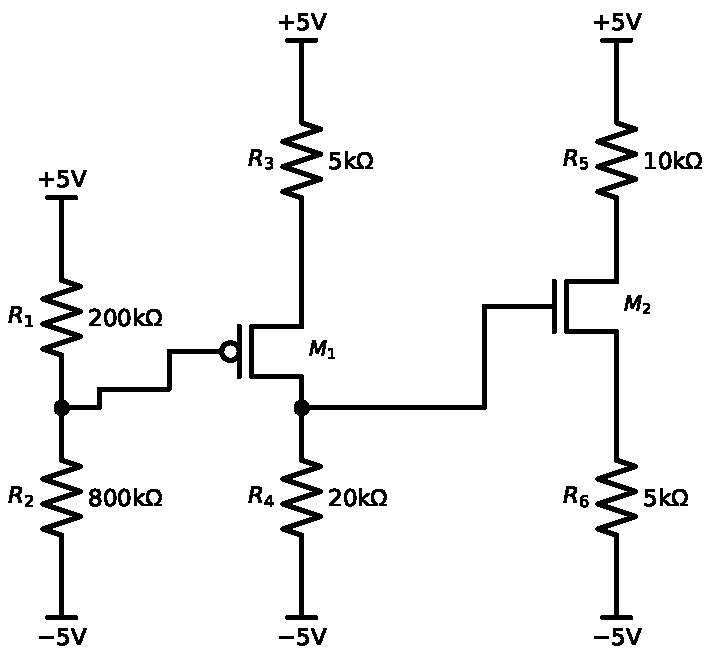
\includegraphics[width=0.9\linewidth,height=6cm,keepaspectratio]{p10_circuit}\end{center}
\solstep{1}{Assumptions}Assume every transistor is active (saturation, tool T1). No current flows into any gate, so gate voltages come from the resistor networks alone.
\solstep{2}{Walk through the circuit}\begin{enumerate}[leftmargin=*,itemsep=3pt]
\item No current flows into a gate ($I_G = 0$), so $V_{G1}$ is set by the divider $R_{1}$--$R_{2}$:\[V_{G1} = -5 + (5 - (-5))\frac{800\,\mathrm{k}}{200\,\mathrm{k} + 800\,\mathrm{k}} = 3\,\mathrm{V}\]
\item KVL from the gate of $M_{1}$ through $V_{SG1}$ and $R_{3}$ ($I_G = 0$, $M_{1}$ assumed active):\[5 - V_{G1} = 2 = V_{SG1} + R_{3}I_{D1}\]\[I_{D1} = \frac{2 - V_{SG1}}{5\,\mathrm{k}} = \frac{400\,\mu }{2}(V_{SG1} - 0.8)^2\]\[1V_{SG1}^2 - 0.6V_{SG1} - 1.36 = 0 \;\Rightarrow\; V_{SG1} = -0.9042\ \text{or}\ 1.504\,\mathrm{V}\]The root $-0.904$\,V is below $|V_t| = 0.8$\,V (the transistor would be off), so $V_{SG1} = 1.504$\,V. Then $I_{D1} = 99.2\,\mu \mathrm{A}$ and $V_{S1} = V_{G1} + V_{SG1} = 4.5\,\mathrm{V}$.
\item $I_{D1} = 99.2\,\mu \mathrm{A}$ flows through $R_{4}$ to $(-5)$: $V_{D1} = (-5) + R_{4}I_{D1} = -5 + 20\,\mathrm{k}\times99.2\,\mu \mathrm{A} = -3.02\,\mathrm{V}$.
\item KVL from the gate of $M_{2}$ through $V_{GS2}$ and $R_{6}$ ($I_G = 0$, $M_{2}$ assumed active):\[V_{D1} - (-5) = 1.983 = V_{GS2} + R_{6}I_{D2}\]\[I_{D2} = \frac{1.983 - V_{GS2}}{5\,\mathrm{k}} = \frac{500\,\mu }{2}(V_{GS2} - 0.8)^2\]\[1.25V_{GS2}^2 - 1V_{GS2} - 1.183 = 0 \;\Rightarrow\; V_{GS2} = -0.652\ \text{or}\ 1.452\,\mathrm{V}\]The root $-0.652$\,V is below $|V_t| = 0.8$\,V (the transistor would be off), so $V_{GS2} = 1.452$\,V. Then $I_{D2} = 106\,\mu \mathrm{A}$ and $V_{S2} = V_{D1} - V_{GS2} = -4.47\,\mathrm{V}$.
\item $I_{D2}$ flows from $5$ through $R_{5}$: $V_{D2} = 5 - R_{5}I_{D2} = 5 - 10\,\mathrm{k}\times106\,\mu \mathrm{A} = 3.94\,\mathrm{V}$.
\end{enumerate}

\solstep{3}{Verify the operating modes}\begin{itemize}[leftmargin=*,itemsep=2pt]
\item $V_{SD1} = V_{S1} - V_{D1} = 4.504 - (-3.017) = 7.52\,\mathrm{V}$ $\ge V_{ov1} = 0.704$\,V $\Rightarrow$ $M_{1}$ is active \checkmark
\item $V_{DS2} = V_{D2} - V_{S2} = 3.937 - (-4.469) = 8.41\,\mathrm{V}$ $\ge V_{ov2} = 0.652$\,V $\Rightarrow$ $M_{2}$ is active \checkmark
\end{itemize}
Unlike the BJT, nothing was neglected here ($I_G = 0$ exactly), so these results are exact for the square-law model: a full nodal solve of the circuit gives the same currents.
\begin{ansbox}
$I_{D1} = 99.2\,\mu \mathrm{A}$,\quad $I_{D2} = 106\,\mu \mathrm{A}$\\[2pt] all transistors active.
\end{ansbox}

\newpage
\subsection*{Solution 5A.11 \hfill Medium}
\begin{center}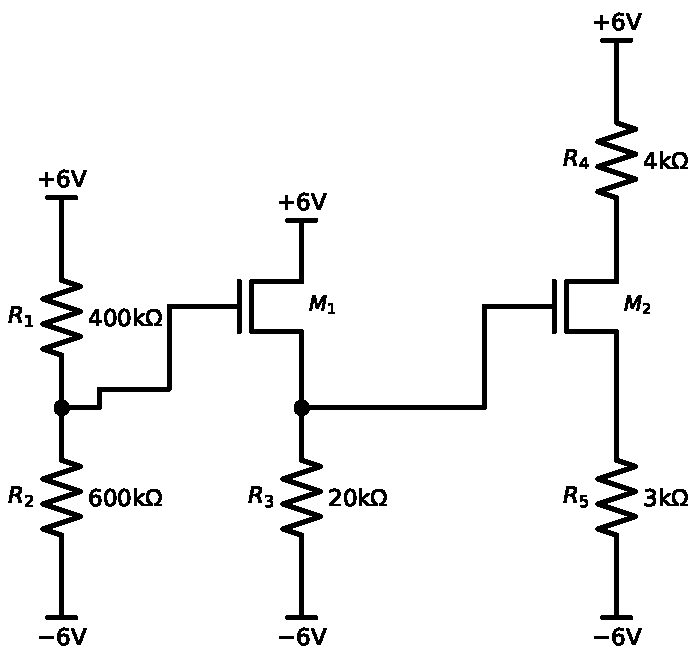
\includegraphics[width=0.9\linewidth,height=6cm,keepaspectratio]{p11_circuit}\end{center}
\solstep{1}{Assumptions}Assume every transistor is active (saturation, tool T1). No current flows into any gate, so gate voltages come from the resistor networks alone.
\solstep{2}{Walk through the circuit}\begin{enumerate}[leftmargin=*,itemsep=3pt]
\item No current flows into a gate ($I_G = 0$), so $V_{G1}$ is set by the divider $R_{1}$--$R_{2}$:\[V_{G1} = -6 + (6 - (-6))\frac{600\,\mathrm{k}}{400\,\mathrm{k} + 600\,\mathrm{k}} = 1.2\,\mathrm{V}\]
\item KVL from the gate of $M_{1}$ through $V_{GS1}$ and $R_{3}$ ($I_G = 0$, $M_{1}$ assumed active):\[V_{G1} - (-6) = 7.2 = V_{GS1} + R_{3}I_{D1}\]\[I_{D1} = \frac{7.2 - V_{GS1}}{20\,\mathrm{k}} = \frac{1.1\,\mathrm{m}}{2}(V_{GS1} - 1.4)^2\]\[11V_{GS1}^2 - 29.8V_{GS1} + 14.36 = 0 \;\Rightarrow\; V_{GS1} = 0.627\ \text{or}\ 2.082\,\mathrm{V}\]The root $0.627$\,V is below $|V_t| = 1.4$\,V (the transistor would be off), so $V_{GS1} = 2.082$\,V. Then $I_{D1} = 256\,\mu \mathrm{A}$ and $V_{S1} = V_{G1} - V_{GS1} = -0.882\,\mathrm{V}$.
\item KVL from the gate of $M_{2}$ through $V_{GS2}$ and $R_{5}$ ($I_G = 0$, $M_{2}$ assumed active):\[V_{S1} - (-6) = 5.118 = V_{GS2} + R_{5}I_{D2}\]\[I_{D2} = \frac{5.118 - V_{GS2}}{3\,\mathrm{k}} = \frac{1.1\,\mathrm{m}}{2}(V_{GS2} - 1.4)^2\]\[1.65V_{GS2}^2 - 3.62V_{GS2} - 1.884 = 0 \;\Rightarrow\; V_{GS2} = -0.4344\ \text{or}\ 2.628\,\mathrm{V}\]The root $-0.434$\,V is below $|V_t| = 1.4$\,V (the transistor would be off), so $V_{GS2} = 2.628$\,V. Then $I_{D2} = 830\,\mu \mathrm{A}$ and $V_{S2} = V_{S1} - V_{GS2} = -3.51\,\mathrm{V}$.
\item $I_{D2}$ flows from $6$ through $R_{4}$: $V_{D2} = 6 - R_{4}I_{D2} = 6 - 4\,\mathrm{k}\times830\,\mu \mathrm{A} = 2.68\,\mathrm{V}$.
\end{enumerate}

\solstep{3}{Verify the operating modes}\begin{itemize}[leftmargin=*,itemsep=2pt]
\item $V_{DS1} = 6 - V_{S1} = 6 - (-0.8821) = 6.88\,\mathrm{V}$ $\ge V_{ov1} = 0.682$\,V $\Rightarrow$ $M_{1}$ is active \checkmark
\item $V_{DS2} = V_{D2} - V_{S2} = 2.681 - (-3.51) = 6.19\,\mathrm{V}$ $\ge V_{ov2} = 1.23$\,V $\Rightarrow$ $M_{2}$ is active \checkmark
\end{itemize}
Unlike the BJT, nothing was neglected here ($I_G = 0$ exactly), so these results are exact for the square-law model: a full nodal solve of the circuit gives the same currents.
\begin{ansbox}
$I_{D1} = 256\,\mu \mathrm{A}$,\quad $I_{D2} = 830\,\mu \mathrm{A}$\\[2pt] all transistors active.
\end{ansbox}

\newpage
\subsection*{Solution 5A.12 \hfill Medium}
\begin{center}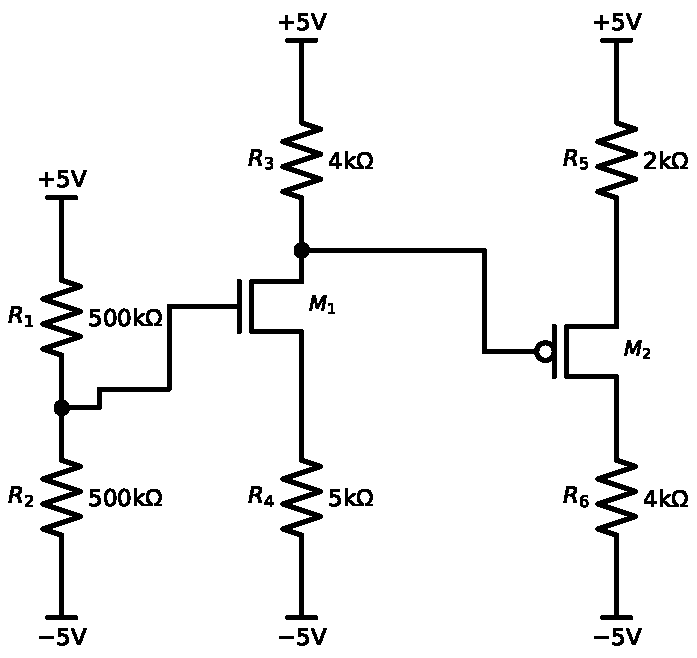
\includegraphics[width=0.9\linewidth,height=6cm,keepaspectratio]{p12_circuit}\end{center}
\solstep{1}{Assumptions}Assume every transistor is active (saturation, tool T1). No current flows into any gate, so gate voltages come from the resistor networks alone.
\solstep{2}{Walk through the circuit}\begin{enumerate}[leftmargin=*,itemsep=3pt]
\item No current flows into a gate ($I_G = 0$), so $V_{G1}$ is set by the divider $R_{1}$--$R_{2}$:\[V_{G1} = -5 + (5 - (-5))\frac{500\,\mathrm{k}}{500\,\mathrm{k} + 500\,\mathrm{k}} = 0\,\mathrm{V}\]
\item KVL from the gate of $M_{1}$ through $V_{GS1}$ and $R_{4}$ ($I_G = 0$, $M_{1}$ assumed active):\[V_{G1} - (-5) = 5 = V_{GS1} + R_{4}I_{D1}\]\[I_{D1} = \frac{5 - V_{GS1}}{5\,\mathrm{k}} = \frac{2\,\mathrm{m}}{2}(V_{GS1} - 1)^2\]\[5V_{GS1}^2 - 9V_{GS1} + 0 = 0 \;\Rightarrow\; V_{GS1} = 0\ \text{or}\ 1.8\,\mathrm{V}\]The root $0$\,V is below $|V_t| = 1$\,V (the transistor would be off), so $V_{GS1} = 1.8$\,V. Then $I_{D1} = 640\,\mu \mathrm{A}$ and $V_{S1} = V_{G1} - V_{GS1} = -1.8\,\mathrm{V}$.
\item $I_{D1}$ flows from $5$ through $R_{3}$: $V_{D1} = 5 - R_{3}I_{D1} = 5 - 4\,\mathrm{k}\times640\,\mu \mathrm{A} = 2.44\,\mathrm{V}$.
\item KVL from the gate of $M_{2}$ through $V_{SG2}$ and $R_{5}$ ($I_G = 0$, $M_{2}$ assumed active):\[5 - V_{D1} = 2.56 = V_{SG2} + R_{5}I_{D2}\]\[I_{D2} = \frac{2.56 - V_{SG2}}{2\,\mathrm{k}} = \frac{1\,\mathrm{m}}{2}(V_{SG2} - 1)^2\]\[1V_{SG2}^2 - 1V_{SG2} - 1.56 = 0 \;\Rightarrow\; V_{SG2} = -0.8454\ \text{or}\ 1.845\,\mathrm{V}\]The root $-0.845$\,V is below $|V_t| = 1$\,V (the transistor would be off), so $V_{SG2} = 1.845$\,V. Then $I_{D2} = 357\,\mu \mathrm{A}$ and $V_{S2} = V_{D1} + V_{SG2} = 4.29\,\mathrm{V}$.
\item $I_{D2} = 357\,\mu \mathrm{A}$ flows through $R_{6}$ to $(-5)$: $V_{D2} = (-5) + R_{6}I_{D2} = -5 + 4\,\mathrm{k}\times357\,\mu \mathrm{A} = -3.57\,\mathrm{V}$.
\end{enumerate}

\solstep{3}{Verify the operating modes}\begin{itemize}[leftmargin=*,itemsep=2pt]
\item $V_{DS1} = V_{D1} - V_{S1} = 2.44 - (-1.8) = 4.24\,\mathrm{V}$ $\ge V_{ov1} = 0.8$\,V $\Rightarrow$ $M_{1}$ is active \checkmark
\item $V_{SD2} = V_{S2} - V_{D2} = 4.285 - (-3.571) = 7.86\,\mathrm{V}$ $\ge V_{ov2} = 0.845$\,V $\Rightarrow$ $M_{2}$ is active \checkmark
\end{itemize}
Unlike the BJT, nothing was neglected here ($I_G = 0$ exactly), so these results are exact for the square-law model: a full nodal solve of the circuit gives the same currents.
\begin{ansbox}
$I_{D1} = 640\,\mu \mathrm{A}$,\quad $I_{D2} = 357\,\mu \mathrm{A}$\\[2pt] all transistors active.
\end{ansbox}

\newpage
\subsection*{Solution 5A.13 \hfill Hard}
\begin{center}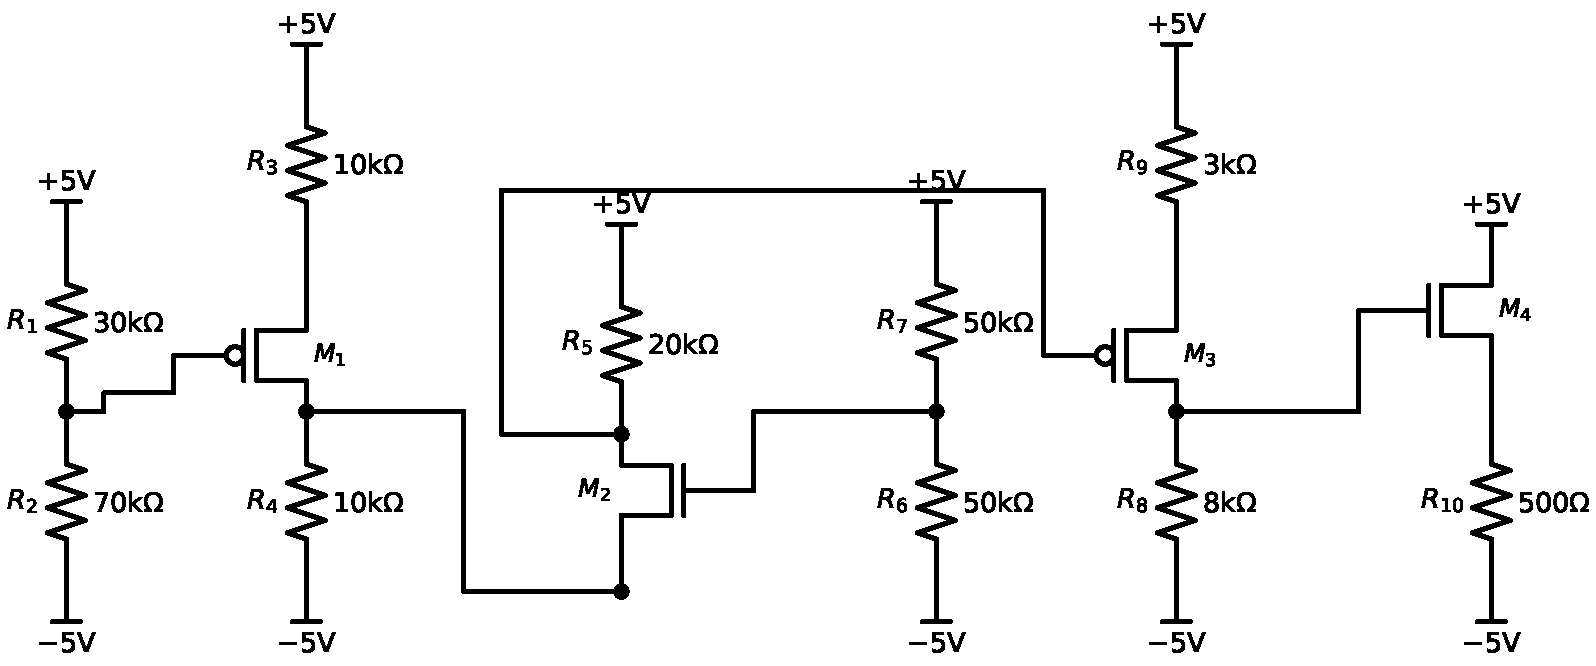
\includegraphics[width=0.9\linewidth,height=6cm,keepaspectratio]{p13_circuit}\end{center}
\solstep{1}{Assumptions}Assume every transistor is active (saturation, tool T1). No current flows into any gate, so gate voltages come from the resistor networks alone.
\solstep{2}{Walk through the circuit}\begin{enumerate}[leftmargin=*,itemsep=3pt]
\item No current flows into a gate ($I_G = 0$), so $V_{G1}$ is set by the divider $R_{1}$--$R_{2}$:\[V_{G1} = -5 + (5 - (-5))\frac{70\,\mathrm{k}}{30\,\mathrm{k} + 70\,\mathrm{k}} = 2\,\mathrm{V}\]
\item No current flows into a gate ($I_G = 0$), so $V_{G2}$ is set by the divider $R_{7}$--$R_{6}$:\[V_{G2} = -5 + (5 - (-5))\frac{50\,\mathrm{k}}{50\,\mathrm{k} + 50\,\mathrm{k}} = 0\,\mathrm{V}\]
\item KVL from the gate of $M_{1}$ through $V_{SG1}$ and $R_{3}$ ($I_G = 0$, $M_{1}$ assumed active):\[5 - V_{G1} = 3 = V_{SG1} + R_{3}I_{D1}\]\[I_{D1} = \frac{3 - V_{SG1}}{10\,\mathrm{k}} = \frac{850\,\mu }{2}(V_{SG1} - 1.3)^2\]\[4.25V_{SG1}^2 - 10.05V_{SG1} + 4.183 = 0 \;\Rightarrow\; V_{SG1} = 0.539\ \text{or}\ 1.826\,\mathrm{V}\]The root $0.539$\,V is below $|V_t| = 1.3$\,V (the transistor would be off), so $V_{SG1} = 1.826$\,V. Then $I_{D1} = 117\,\mu \mathrm{A}$ and $V_{S1} = V_{G1} + V_{SG1} = 3.83\,\mathrm{V}$.
\item KVL from the gate of $M_{2}$ through $V_{GS2}$ and $R_{4}$ ($I_G = 0$, $M_{2}$ assumed active):\[V_{G2} - (-5) = 5 = V_{GS2} + R_{4}(I_{D2} + I_{D1})\]\[I_{D2} = \frac{5 - 10\,\mathrm{k}\times117\,\mu \mathrm{A} - V_{GS2}}{10\,\mathrm{k}} = \frac{1.1\,\mathrm{m}}{2}(V_{GS2} - 1.4)^2\]\[5.5V_{GS2}^2 - 14.4V_{GS2} + 6.954 = 0 \;\Rightarrow\; V_{GS2} = 0.6388\ \text{or}\ 1.979\,\mathrm{V}\]The root $0.639$\,V is below $|V_t| = 1.4$\,V (the transistor would be off), so $V_{GS2} = 1.979$\,V. Then $I_{D2} = 185\,\mu \mathrm{A}$ and $V_{D1} = V_{G2} - V_{GS2} = -1.98\,\mathrm{V}$.
\item $I_{D2}$ flows from $5$ through $R_{5}$: $V_{D2} = 5 - R_{5}I_{D2} = 5 - 20\,\mathrm{k}\times185\,\mu \mathrm{A} = 1.31\,\mathrm{V}$.
\item KVL from the gate of $M_{3}$ through $V_{SG3}$ and $R_{9}$ ($I_G = 0$, $M_{3}$ assumed active):\[5 - V_{D2} = 3.693 = V_{SG3} + R_{9}I_{D3}\]\[I_{D3} = \frac{3.693 - V_{SG3}}{3\,\mathrm{k}} = \frac{850\,\mu }{2}(V_{SG3} - 1.3)^2\]\[1.275V_{SG3}^2 - 2.315V_{SG3} - 1.538 = 0 \;\Rightarrow\; V_{SG3} = -0.517\ \text{or}\ 2.333\,\mathrm{V}\]The root $-0.517$\,V is below $|V_t| = 1.3$\,V (the transistor would be off), so $V_{SG3} = 2.333$\,V. Then $I_{D3} = 453\,\mu \mathrm{A}$ and $V_{S3} = V_{D2} + V_{SG3} = 3.64\,\mathrm{V}$.
\item $I_{D3} = 453\,\mu \mathrm{A}$ flows through $R_{8}$ to $(-5)$: $V_{D3} = (-5) + R_{8}I_{D3} = -5 + 8\,\mathrm{k}\times453\,\mu \mathrm{A} = -1.37\,\mathrm{V}$.
\item KVL from the gate of $M_{4}$ through $V_{GS4}$ and $R_{10}$ ($I_G = 0$, $M_{4}$ assumed active):\[V_{D3} - (-5) = 3.626 = V_{GS4} + R_{10}I_{D4}\]\[I_{D4} = \frac{3.626 - V_{GS4}}{500} = \frac{1.1\,\mathrm{m}}{2}(V_{GS4} - 1.4)^2\]\[0.275V_{GS4}^2 + 0.23V_{GS4} - 3.087 = 0 \;\Rightarrow\; V_{GS4} = -3.795\ \text{or}\ 2.958\,\mathrm{V}\]The root $-3.79$\,V is below $|V_t| = 1.4$\,V (the transistor would be off), so $V_{GS4} = 2.958$\,V. Then $I_{D4} = 1.34\,\mathrm{m}\mathrm{A}$ and $V_{S4} = V_{D3} - V_{GS4} = -4.33\,\mathrm{V}$.
\end{enumerate}

\solstep{3}{Verify the operating modes}\begin{itemize}[leftmargin=*,itemsep=2pt]
\item $V_{SD1} = V_{S1} - V_{D1} = 3.826 - (-1.979) = 5.81\,\mathrm{V}$ $\ge V_{ov1} = 0.526$\,V $\Rightarrow$ $M_{1}$ is active \checkmark
\item $V_{DS2} = V_{D2} - V_{D1} = 1.307 - (-1.979) = 3.29\,\mathrm{V}$ $\ge V_{ov2} = 0.579$\,V $\Rightarrow$ $M_{2}$ is active \checkmark
\item $V_{SD3} = V_{S3} - V_{D3} = 3.64 - (-1.374) = 5.01\,\mathrm{V}$ $\ge V_{ov3} = 1.03$\,V $\Rightarrow$ $M_{3}$ is active \checkmark
\item $V_{DS4} = 5 - V_{S4} = 5 - (-4.332) = 9.33\,\mathrm{V}$ $\ge V_{ov4} = 1.56$\,V $\Rightarrow$ $M_{4}$ is active \checkmark
\end{itemize}
Unlike the BJT, nothing was neglected here ($I_G = 0$ exactly), so these results are exact for the square-law model: a full nodal solve of the circuit gives the same currents.
\begin{ansbox}
$I_{D1} = 117\,\mu \mathrm{A}$,\quad $I_{D2} = 185\,\mu \mathrm{A}$,\quad $I_{D3} = 453\,\mu \mathrm{A}$,\quad $I_{D4} = 1.34\,\mathrm{m}\mathrm{A}$\\[2pt] all transistors active.
\end{ansbox}

\newpage
\subsection*{Solution 5A.14 \hfill Hard}
\begin{center}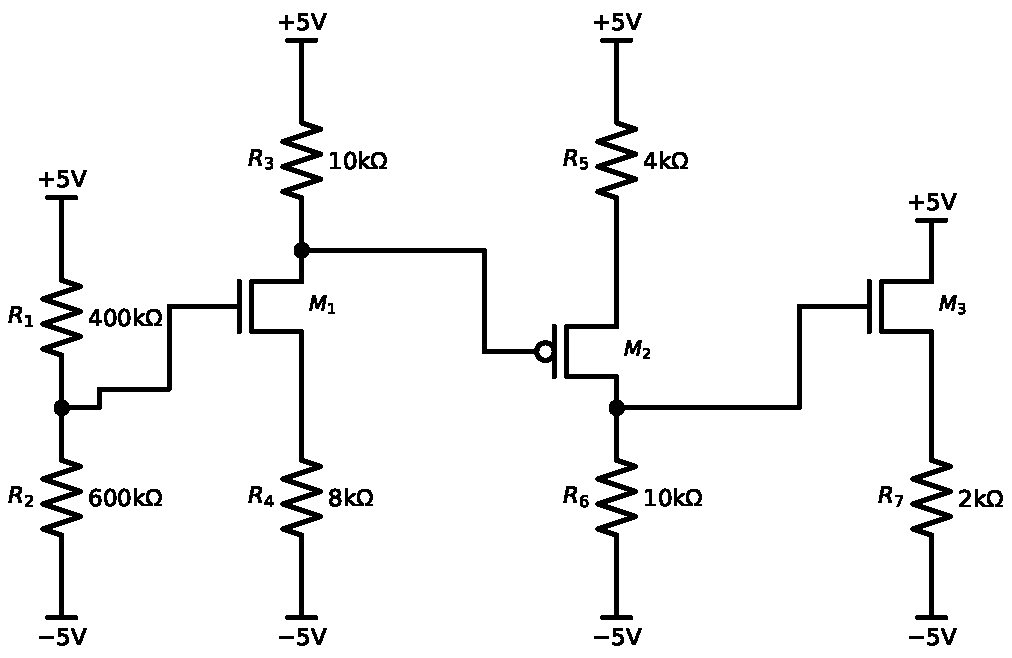
\includegraphics[width=0.9\linewidth,height=6cm,keepaspectratio]{p14_circuit}\end{center}
\solstep{1}{Assumptions}Assume every transistor is active (saturation, tool T1). No current flows into any gate, so gate voltages come from the resistor networks alone.
\solstep{2}{Walk through the circuit}\begin{enumerate}[leftmargin=*,itemsep=3pt]
\item No current flows into a gate ($I_G = 0$), so $V_{G1}$ is set by the divider $R_{1}$--$R_{2}$:\[V_{G1} = -5 + (5 - (-5))\frac{600\,\mathrm{k}}{400\,\mathrm{k} + 600\,\mathrm{k}} = 1\,\mathrm{V}\]
\item KVL from the gate of $M_{1}$ through $V_{GS1}$ and $R_{4}$ ($I_G = 0$, $M_{1}$ assumed active):\[V_{G1} - (-5) = 6 = V_{GS1} + R_{4}I_{D1}\]\[I_{D1} = \frac{6 - V_{GS1}}{8\,\mathrm{k}} = \frac{1.1\,\mathrm{m}}{2}(V_{GS1} - 1.4)^2\]\[4.4V_{GS1}^2 - 11.32V_{GS1} + 2.624 = 0 \;\Rightarrow\; V_{GS1} = 0.2576\ \text{or}\ 2.315\,\mathrm{V}\]The root $0.258$\,V is below $|V_t| = 1.4$\,V (the transistor would be off), so $V_{GS1} = 2.315$\,V. Then $I_{D1} = 461\,\mu \mathrm{A}$ and $V_{S1} = V_{G1} - V_{GS1} = -1.32\,\mathrm{V}$.
\item $I_{D1}$ flows from $5$ through $R_{3}$: $V_{D1} = 5 - R_{3}I_{D1} = 5 - 10\,\mathrm{k}\times461\,\mu \mathrm{A} = 0.394\,\mathrm{V}$.
\item KVL from the gate of $M_{2}$ through $V_{SG2}$ and $R_{5}$ ($I_G = 0$, $M_{2}$ assumed active):\[5 - V_{D1} = 4.606 = V_{SG2} + R_{5}I_{D2}\]\[I_{D2} = \frac{4.606 - V_{SG2}}{4\,\mathrm{k}} = \frac{850\,\mu }{2}(V_{SG2} - 1.3)^2\]\[1.7V_{SG2}^2 - 3.42V_{SG2} - 1.733 = 0 \;\Rightarrow\; V_{SG2} = -0.4193\ \text{or}\ 2.431\,\mathrm{V}\]The root $-0.419$\,V is below $|V_t| = 1.3$\,V (the transistor would be off), so $V_{SG2} = 2.431$\,V. Then $I_{D2} = 544\,\mu \mathrm{A}$ and $V_{S2} = V_{D1} + V_{SG2} = 2.83\,\mathrm{V}$.
\item $I_{D2} = 544\,\mu \mathrm{A}$ flows through $R_{6}$ to $(-5)$: $V_{D2} = (-5) + R_{6}I_{D2} = -5 + 10\,\mathrm{k}\times544\,\mu \mathrm{A} = 0.437\,\mathrm{V}$.
\item KVL from the gate of $M_{3}$ through $V_{GS3}$ and $R_{7}$ ($I_G = 0$, $M_{3}$ assumed active):\[V_{D2} - (-5) = 5.437 = V_{GS3} + R_{7}I_{D3}\]\[I_{D3} = \frac{5.437 - V_{GS3}}{2\,\mathrm{k}} = \frac{1.1\,\mathrm{m}}{2}(V_{GS3} - 1.4)^2\]\[1.1V_{GS3}^2 - 2.08V_{GS3} - 3.281 = 0 \;\Rightarrow\; V_{GS3} = -1.024\ \text{or}\ 2.914\,\mathrm{V}\]The root $-1.02$\,V is below $|V_t| = 1.4$\,V (the transistor would be off), so $V_{GS3} = 2.914$\,V. Then $I_{D3} = 1.26\,\mathrm{m}\mathrm{A}$ and $V_{S3} = V_{D2} - V_{GS3} = -2.48\,\mathrm{V}$.
\end{enumerate}

\solstep{3}{Verify the operating modes}\begin{itemize}[leftmargin=*,itemsep=2pt]
\item $V_{DS1} = V_{D1} - V_{S1} = 0.3939 - (-1.315) = 1.71\,\mathrm{V}$ $\ge V_{ov1} = 0.915$\,V $\Rightarrow$ $M_{1}$ is active \checkmark
\item $V_{SD2} = V_{S2} - V_{D2} = 2.825 - 0.4374 = 2.39\,\mathrm{V}$ $\ge V_{ov2} = 1.13$\,V $\Rightarrow$ $M_{2}$ is active \checkmark
\item $V_{DS3} = 5 - V_{S3} = 5 - (-2.477) = 7.48\,\mathrm{V}$ $\ge V_{ov3} = 1.51$\,V $\Rightarrow$ $M_{3}$ is active \checkmark
\end{itemize}
Unlike the BJT, nothing was neglected here ($I_G = 0$ exactly), so these results are exact for the square-law model: a full nodal solve of the circuit gives the same currents.
\begin{ansbox}
$I_{D1} = 461\,\mu \mathrm{A}$,\quad $I_{D2} = 544\,\mu \mathrm{A}$,\quad $I_{D3} = 1.26\,\mathrm{m}\mathrm{A}$\\[2pt] all transistors active.
\end{ansbox}

\newpage
\subsection*{Solution 5A.15 \hfill Hard}
\begin{center}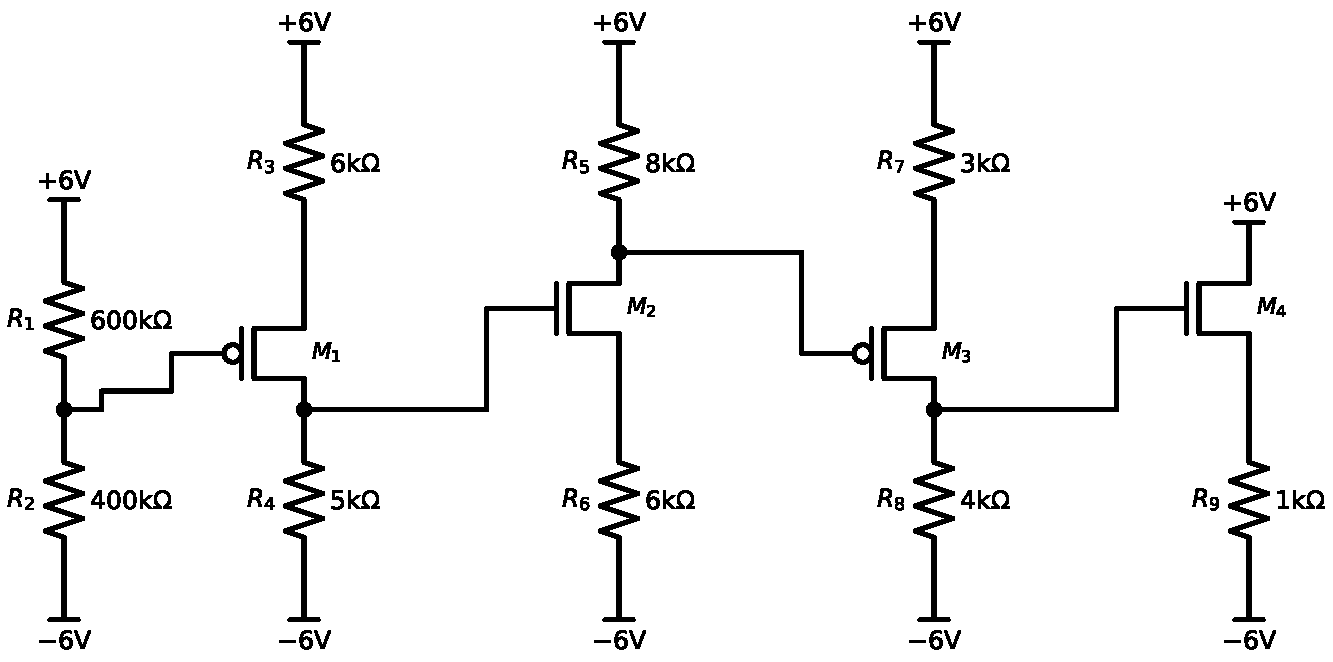
\includegraphics[width=0.9\linewidth,height=6cm,keepaspectratio]{p15_circuit}\end{center}
\solstep{1}{Assumptions}Assume every transistor is active (saturation, tool T1). No current flows into any gate, so gate voltages come from the resistor networks alone.
\solstep{2}{Walk through the circuit}\begin{enumerate}[leftmargin=*,itemsep=3pt]
\item No current flows into a gate ($I_G = 0$), so $V_{G1}$ is set by the divider $R_{1}$--$R_{2}$:\[V_{G1} = -6 + (6 - (-6))\frac{400\,\mathrm{k}}{600\,\mathrm{k} + 400\,\mathrm{k}} = -1.2\,\mathrm{V}\]
\item KVL from the gate of $M_{1}$ through $V_{SG1}$ and $R_{3}$ ($I_G = 0$, $M_{1}$ assumed active):\[6 - V_{G1} = 7.2 = V_{SG1} + R_{3}I_{D1}\]\[I_{D1} = \frac{7.2 - V_{SG1}}{6\,\mathrm{k}} = \frac{1\,\mathrm{m}}{2}(V_{SG1} - 1)^2\]\[3V_{SG1}^2 - 5V_{SG1} - 4.2 = 0 \;\Rightarrow\; V_{SG1} = -0.6139\ \text{or}\ 2.281\,\mathrm{V}\]The root $-0.614$\,V is below $|V_t| = 1$\,V (the transistor would be off), so $V_{SG1} = 2.281$\,V. Then $I_{D1} = 820\,\mu \mathrm{A}$ and $V_{S1} = V_{G1} + V_{SG1} = 1.08\,\mathrm{V}$.
\item $I_{D1} = 820\,\mu \mathrm{A}$ flows through $R_{4}$ to $(-6)$: $V_{D1} = (-6) + R_{4}I_{D1} = -6 + 5\,\mathrm{k}\times820\,\mu \mathrm{A} = -1.9\,\mathrm{V}$.
\item KVL from the gate of $M_{2}$ through $V_{GS2}$ and $R_{6}$ ($I_G = 0$, $M_{2}$ assumed active):\[V_{D1} - (-6) = 4.1 = V_{GS2} + R_{6}I_{D2}\]\[I_{D2} = \frac{4.1 - V_{GS2}}{6\,\mathrm{k}} = \frac{2\,\mathrm{m}}{2}(V_{GS2} - 1)^2\]\[6V_{GS2}^2 - 11V_{GS2} + 1.9 = 0 \;\Rightarrow\; V_{GS2} = 0.1931\ \text{or}\ 1.64\,\mathrm{V}\]The root $0.193$\,V is below $|V_t| = 1$\,V (the transistor would be off), so $V_{GS2} = 1.64$\,V. Then $I_{D2} = 410\,\mu \mathrm{A}$ and $V_{S2} = V_{D1} - V_{GS2} = -3.54\,\mathrm{V}$.
\item $I_{D2}$ flows from $6$ through $R_{5}$: $V_{D2} = 6 - R_{5}I_{D2} = 6 - 8\,\mathrm{k}\times410\,\mu \mathrm{A} = 2.72\,\mathrm{V}$.
\item KVL from the gate of $M_{3}$ through $V_{SG3}$ and $R_{7}$ ($I_G = 0$, $M_{3}$ assumed active):\[6 - V_{D2} = 3.279 = V_{SG3} + R_{7}I_{D3}\]\[I_{D3} = \frac{3.279 - V_{SG3}}{3\,\mathrm{k}} = \frac{1\,\mathrm{m}}{2}(V_{SG3} - 1)^2\]\[1.5V_{SG3}^2 - 2V_{SG3} - 1.779 = 0 \;\Rightarrow\; V_{SG3} = -0.6102\ \text{or}\ 1.944\,\mathrm{V}\]The root $-0.61$\,V is below $|V_t| = 1$\,V (the transistor would be off), so $V_{SG3} = 1.944$\,V. Then $I_{D3} = 445\,\mu \mathrm{A}$ and $V_{S3} = V_{D2} + V_{SG3} = 4.66\,\mathrm{V}$.
\item $I_{D3} = 445\,\mu \mathrm{A}$ flows through $R_{8}$ to $(-6)$: $V_{D3} = (-6) + R_{8}I_{D3} = -6 + 4\,\mathrm{k}\times445\,\mu \mathrm{A} = -4.22\,\mathrm{V}$.
\item KVL from the gate of $M_{4}$ through $V_{GS4}$ and $R_{9}$ ($I_G = 0$, $M_{4}$ assumed active):\[V_{D3} - (-6) = 1.781 = V_{GS4} + R_{9}I_{D4}\]\[I_{D4} = \frac{1.781 - V_{GS4}}{1\,\mathrm{k}} = \frac{2\,\mathrm{m}}{2}(V_{GS4} - 1)^2\]\[1V_{GS4}^2 - 1V_{GS4} - 0.7807 = 0 \;\Rightarrow\; V_{GS4} = -0.5152\ \text{or}\ 1.515\,\mathrm{V}\]The root $-0.515$\,V is below $|V_t| = 1$\,V (the transistor would be off), so $V_{GS4} = 1.515$\,V. Then $I_{D4} = 265\,\mu \mathrm{A}$ and $V_{S4} = V_{D3} - V_{GS4} = -5.73\,\mathrm{V}$.
\end{enumerate}

\solstep{3}{Verify the operating modes}\begin{itemize}[leftmargin=*,itemsep=2pt]
\item $V_{SD1} = V_{S1} - V_{D1} = 1.081 - (-1.9) = 2.98\,\mathrm{V}$ $\ge V_{ov1} = 1.28$\,V $\Rightarrow$ $M_{1}$ is active \checkmark
\item $V_{DS2} = V_{D2} - V_{S2} = 2.721 - (-3.541) = 6.26\,\mathrm{V}$ $\ge V_{ov2} = 0.64$\,V $\Rightarrow$ $M_{2}$ is active \checkmark
\item $V_{SD3} = V_{S3} - V_{D3} = 4.664 - (-4.219) = 8.88\,\mathrm{V}$ $\ge V_{ov3} = 0.944$\,V $\Rightarrow$ $M_{3}$ is active \checkmark
\item $V_{DS4} = 6 - V_{S4} = 6 - (-5.735) = 11.7\,\mathrm{V}$ $\ge V_{ov4} = 0.515$\,V $\Rightarrow$ $M_{4}$ is active \checkmark
\end{itemize}
Unlike the BJT, nothing was neglected here ($I_G = 0$ exactly), so these results are exact for the square-law model: a full nodal solve of the circuit gives the same currents.
\begin{ansbox}
$I_{D1} = 820\,\mu \mathrm{A}$,\quad $I_{D2} = 410\,\mu \mathrm{A}$,\quad $I_{D3} = 445\,\mu \mathrm{A}$,\quad $I_{D4} = 265\,\mu \mathrm{A}$\\[2pt] all transistors active.
\end{ansbox}

\newpage
\subsection*{Solution 5A.16 \hfill Hard}
\begin{center}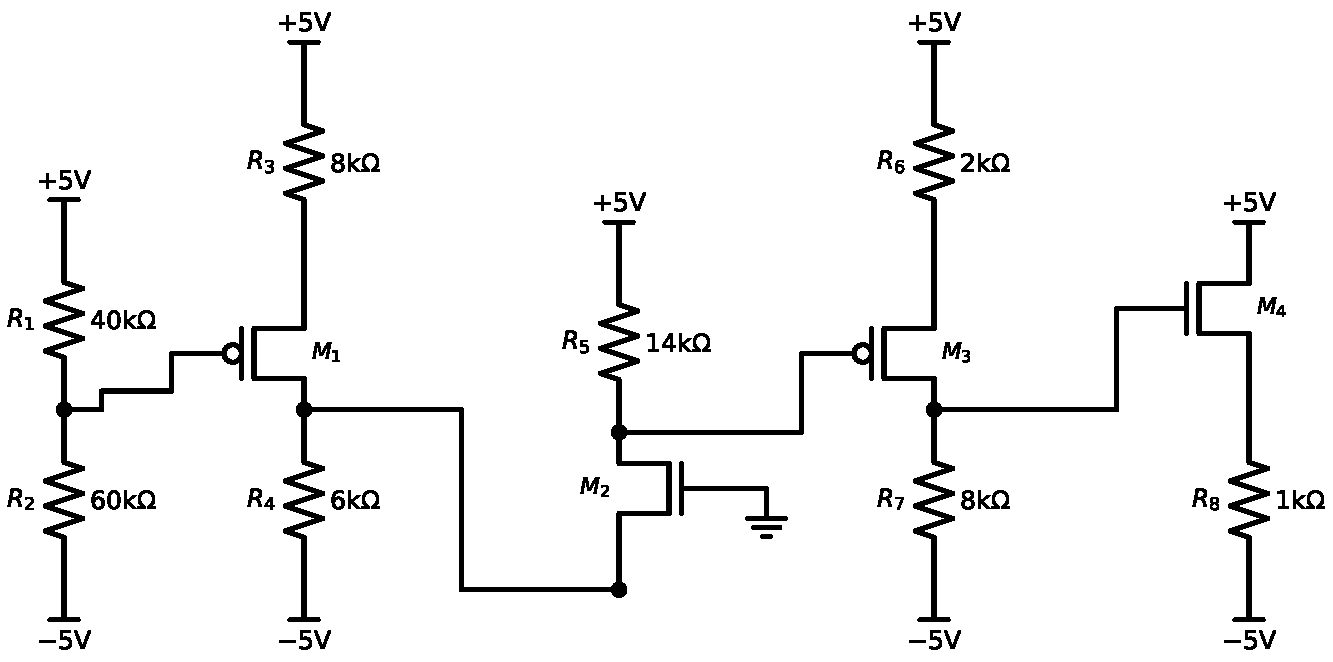
\includegraphics[width=0.9\linewidth,height=6cm,keepaspectratio]{p16_circuit}\end{center}
\solstep{1}{Assumptions}Assume every transistor is active (saturation, tool T1). No current flows into any gate, so gate voltages come from the resistor networks alone.
\solstep{2}{Walk through the circuit}\begin{enumerate}[leftmargin=*,itemsep=3pt]
\item No current flows into a gate ($I_G = 0$), so $V_{G1}$ is set by the divider $R_{1}$--$R_{2}$:\[V_{G1} = -5 + (5 - (-5))\frac{60\,\mathrm{k}}{40\,\mathrm{k} + 60\,\mathrm{k}} = 1\,\mathrm{V}\]
\item KVL from the gate of $M_{1}$ through $V_{SG1}$ and $R_{3}$ ($I_G = 0$, $M_{1}$ assumed active):\[5 - V_{G1} = 4 = V_{SG1} + R_{3}I_{D1}\]\[I_{D1} = \frac{4 - V_{SG1}}{8\,\mathrm{k}} = \frac{850\,\mu }{2}(V_{SG1} - 1.3)^2\]\[3.4V_{SG1}^2 - 7.84V_{SG1} + 1.746 = 0 \;\Rightarrow\; V_{SG1} = 0.2498\ \text{or}\ 2.056\,\mathrm{V}\]The root $0.25$\,V is below $|V_t| = 1.3$\,V (the transistor would be off), so $V_{SG1} = 2.056$\,V. Then $I_{D1} = 243\,\mu \mathrm{A}$ and $V_{S1} = V_{G1} + V_{SG1} = 3.06\,\mathrm{V}$.
\item KVL from the gate of $M_{2}$ through $V_{GS2}$ and $R_{4}$ ($I_G = 0$, $M_{2}$ assumed active):\[0 - (-5) = 5 = V_{GS2} + R_{4}(I_{D2} + I_{D1})\]\[I_{D2} = \frac{5 - 6\,\mathrm{k}\times243\,\mu \mathrm{A} - V_{GS2}}{6\,\mathrm{k}} = \frac{1.1\,\mathrm{m}}{2}(V_{GS2} - 1.4)^2\]\[3.3V_{GS2}^2 - 8.24V_{GS2} + 2.926 = 0 \;\Rightarrow\; V_{GS2} = 0.4287\ \text{or}\ 2.068\,\mathrm{V}\]The root $0.429$\,V is below $|V_t| = 1.4$\,V (the transistor would be off), so $V_{GS2} = 2.068$\,V. Then $I_{D2} = 246\,\mu \mathrm{A}$ and $V_{D1} = 0 - V_{GS2} = -2.07\,\mathrm{V}$.
\item $I_{D2}$ flows from $5$ through $R_{5}$: $V_{D2} = 5 - R_{5}I_{D2} = 5 - 14\,\mathrm{k}\times246\,\mu \mathrm{A} = 1.56\,\mathrm{V}$.
\item KVL from the gate of $M_{3}$ through $V_{SG3}$ and $R_{6}$ ($I_G = 0$, $M_{3}$ assumed active):\[5 - V_{D2} = 3.439 = V_{SG3} + R_{6}I_{D3}\]\[I_{D3} = \frac{3.439 - V_{SG3}}{2\,\mathrm{k}} = \frac{850\,\mu }{2}(V_{SG3} - 1.3)^2\]\[0.85V_{SG3}^2 - 1.21V_{SG3} - 2.002 = 0 \;\Rightarrow\; V_{SG3} = -0.9801\ \text{or}\ 2.404\,\mathrm{V}\]The root $-0.98$\,V is below $|V_t| = 1.3$\,V (the transistor would be off), so $V_{SG3} = 2.404$\,V. Then $I_{D3} = 518\,\mu \mathrm{A}$ and $V_{S3} = V_{D2} + V_{SG3} = 3.96\,\mathrm{V}$.
\item $I_{D3} = 518\,\mu \mathrm{A}$ flows through $R_{7}$ to $(-5)$: $V_{D3} = (-5) + R_{7}I_{D3} = -5 + 8\,\mathrm{k}\times518\,\mu \mathrm{A} = -0.859\,\mathrm{V}$.
\item KVL from the gate of $M_{4}$ through $V_{GS4}$ and $R_{8}$ ($I_G = 0$, $M_{4}$ assumed active):\[V_{D3} - (-5) = 4.141 = V_{GS4} + R_{8}I_{D4}\]\[I_{D4} = \frac{4.141 - V_{GS4}}{1\,\mathrm{k}} = \frac{1.1\,\mathrm{m}}{2}(V_{GS4} - 1.4)^2\]\[0.55V_{GS4}^2 - 0.54V_{GS4} - 3.063 = 0 \;\Rightarrow\; V_{GS4} = -1.92\ \text{or}\ 2.901\,\mathrm{V}\]The root $-1.92$\,V is below $|V_t| = 1.4$\,V (the transistor would be off), so $V_{GS4} = 2.901$\,V. Then $I_{D4} = 1.24\,\mathrm{m}\mathrm{A}$ and $V_{S4} = V_{D3} - V_{GS4} = -3.76\,\mathrm{V}$.
\end{enumerate}

\solstep{3}{Verify the operating modes}\begin{itemize}[leftmargin=*,itemsep=2pt]
\item $V_{SD1} = V_{S1} - V_{D1} = 3.056 - (-2.068) = 5.12\,\mathrm{V}$ $\ge V_{ov1} = 0.756$\,V $\Rightarrow$ $M_{1}$ is active \checkmark
\item $V_{DS2} = V_{D2} - V_{D1} = 1.561 - (-2.068) = 3.63\,\mathrm{V}$ $\ge V_{ov2} = 0.668$\,V $\Rightarrow$ $M_{2}$ is active \checkmark
\item $V_{SD3} = V_{S3} - V_{D3} = 3.965 - (-0.8589) = 4.82\,\mathrm{V}$ $\ge V_{ov3} = 1.1$\,V $\Rightarrow$ $M_{3}$ is active \checkmark
\item $V_{DS4} = 5 - V_{S4} = 5 - (-3.76) = 8.76\,\mathrm{V}$ $\ge V_{ov4} = 1.5$\,V $\Rightarrow$ $M_{4}$ is active \checkmark
\end{itemize}
Unlike the BJT, nothing was neglected here ($I_G = 0$ exactly), so these results are exact for the square-law model: a full nodal solve of the circuit gives the same currents.
\begin{ansbox}
$I_{D1} = 243\,\mu \mathrm{A}$,\quad $I_{D2} = 246\,\mu \mathrm{A}$,\quad $I_{D3} = 518\,\mu \mathrm{A}$,\quad $I_{D4} = 1.24\,\mathrm{m}\mathrm{A}$\\[2pt] all transistors active.
\end{ansbox}

\newpage
\subsection*{Solution 5A.17 \hfill Hard}
\begin{center}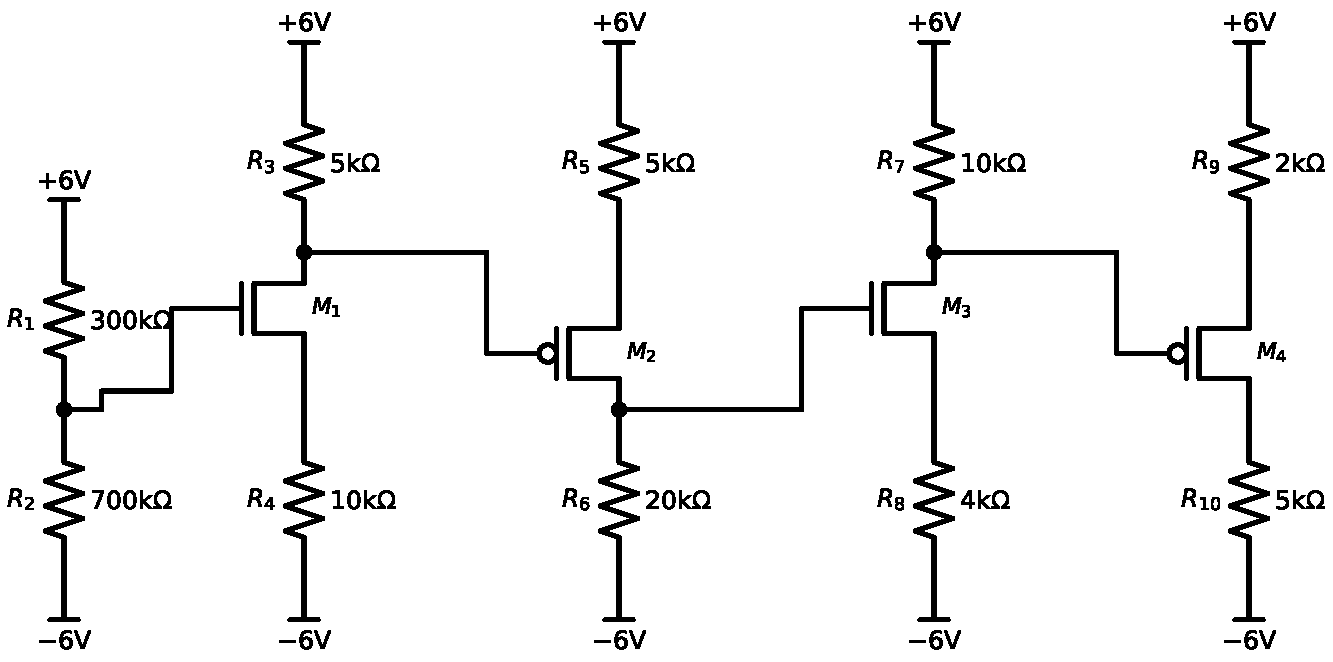
\includegraphics[width=0.9\linewidth,height=6cm,keepaspectratio]{p17_circuit}\end{center}
\solstep{1}{Assumptions}Assume every transistor is active (saturation, tool T1). No current flows into any gate, so gate voltages come from the resistor networks alone.
\solstep{2}{Walk through the circuit}\begin{enumerate}[leftmargin=*,itemsep=3pt]
\item No current flows into a gate ($I_G = 0$), so $V_{G1}$ is set by the divider $R_{1}$--$R_{2}$:\[V_{G1} = -6 + (6 - (-6))\frac{700\,\mathrm{k}}{300\,\mathrm{k} + 700\,\mathrm{k}} = 2.4\,\mathrm{V}\]
\item KVL from the gate of $M_{1}$ through $V_{GS1}$ and $R_{4}$ ($I_G = 0$, $M_{1}$ assumed active):\[V_{G1} - (-6) = 8.4 = V_{GS1} + R_{4}I_{D1}\]\[I_{D1} = \frac{8.4 - V_{GS1}}{10\,\mathrm{k}} = \frac{500\,\mu }{2}(V_{GS1} - 0.8)^2\]\[2.5V_{GS1}^2 - 3V_{GS1} - 6.8 = 0 \;\Rightarrow\; V_{GS1} = -1.155\ \text{or}\ 2.355\,\mathrm{V}\]The root $-1.15$\,V is below $|V_t| = 0.8$\,V (the transistor would be off), so $V_{GS1} = 2.355$\,V. Then $I_{D1} = 605\,\mu \mathrm{A}$ and $V_{S1} = V_{G1} - V_{GS1} = 0.045\,\mathrm{V}$.
\item $I_{D1}$ flows from $6$ through $R_{3}$: $V_{D1} = 6 - R_{3}I_{D1} = 6 - 5\,\mathrm{k}\times605\,\mu \mathrm{A} = 2.98\,\mathrm{V}$.
\item KVL from the gate of $M_{2}$ through $V_{SG2}$ and $R_{5}$ ($I_G = 0$, $M_{2}$ assumed active):\[6 - V_{D1} = 3.023 = V_{SG2} + R_{5}I_{D2}\]\[I_{D2} = \frac{3.023 - V_{SG2}}{5\,\mathrm{k}} = \frac{400\,\mu }{2}(V_{SG2} - 0.8)^2\]\[1V_{SG2}^2 - 0.6V_{SG2} - 2.383 = 0 \;\Rightarrow\; V_{SG2} = -1.272\ \text{or}\ 1.872\,\mathrm{V}\]The root $-1.27$\,V is below $|V_t| = 0.8$\,V (the transistor would be off), so $V_{SG2} = 1.872$\,V. Then $I_{D2} = 230\,\mu \mathrm{A}$ and $V_{S2} = V_{D1} + V_{SG2} = 4.85\,\mathrm{V}$.
\item $I_{D2} = 230\,\mu \mathrm{A}$ flows through $R_{6}$ to $(-6)$: $V_{D2} = (-6) + R_{6}I_{D2} = -6 + 20\,\mathrm{k}\times230\,\mu \mathrm{A} = -1.4\,\mathrm{V}$.
\item KVL from the gate of $M_{3}$ through $V_{GS3}$ and $R_{8}$ ($I_G = 0$, $M_{3}$ assumed active):\[V_{D2} - (-6) = 4.6 = V_{GS3} + R_{8}I_{D3}\]\[I_{D3} = \frac{4.6 - V_{GS3}}{4\,\mathrm{k}} = \frac{500\,\mu }{2}(V_{GS3} - 0.8)^2\]\[1V_{GS3}^2 - 0.6V_{GS3} - 3.96 = 0 \;\Rightarrow\; V_{GS3} = -1.713\ \text{or}\ 2.313\,\mathrm{V}\]The root $-1.71$\,V is below $|V_t| = 0.8$\,V (the transistor would be off), so $V_{GS3} = 2.313$\,V. Then $I_{D3} = 572\,\mu \mathrm{A}$ and $V_{S3} = V_{D2} - V_{GS3} = -3.71\,\mathrm{V}$.
\item $I_{D3}$ flows from $6$ through $R_{7}$: $V_{D3} = 6 - R_{7}I_{D3} = 6 - 10\,\mathrm{k}\times572\,\mu \mathrm{A} = 0.281\,\mathrm{V}$.
\item KVL from the gate of $M_{4}$ through $V_{SG4}$ and $R_{9}$ ($I_G = 0$, $M_{4}$ assumed active):\[6 - V_{D3} = 5.719 = V_{SG4} + R_{9}I_{D4}\]\[I_{D4} = \frac{5.719 - V_{SG4}}{2\,\mathrm{k}} = \frac{400\,\mu }{2}(V_{SG4} - 0.8)^2\]\[0.4V_{SG4}^2 + 0.36V_{SG4} - 5.463 = 0 \;\Rightarrow\; V_{SG4} = -4.173\ \text{or}\ 3.273\,\mathrm{V}\]The root $-4.17$\,V is below $|V_t| = 0.8$\,V (the transistor would be off), so $V_{SG4} = 3.273$\,V. Then $I_{D4} = 1.22\,\mathrm{m}\mathrm{A}$ and $V_{S4} = V_{D3} + V_{SG4} = 3.55\,\mathrm{V}$.
\item $I_{D4} = 1.22\,\mathrm{m}\mathrm{A}$ flows through $R_{10}$ to $(-6)$: $V_{D4} = (-6) + R_{10}I_{D4} = -6 + 5\,\mathrm{k}\times1.22\,\mathrm{m}\mathrm{A} = 0.116\,\mathrm{V}$.
\end{enumerate}

\solstep{3}{Verify the operating modes}\begin{itemize}[leftmargin=*,itemsep=2pt]
\item $V_{DS1} = V_{D1} - V_{S1} = 2.977 - 0.04501 = 2.93\,\mathrm{V}$ $\ge V_{ov1} = 1.55$\,V $\Rightarrow$ $M_{1}$ is active \checkmark
\item $V_{SD2} = V_{S2} - V_{D2} = 4.85 - (-1.4) = 6.25\,\mathrm{V}$ $\ge V_{ov2} = 1.07$\,V $\Rightarrow$ $M_{2}$ is active \checkmark
\item $V_{DS3} = V_{D3} - V_{S3} = 0.2805 - (-3.712) = 3.99\,\mathrm{V}$ $\ge V_{ov3} = 1.51$\,V $\Rightarrow$ $M_{3}$ is active \checkmark
\item $V_{SD4} = V_{S4} - V_{D4} = 3.554 - 0.116 = 3.44\,\mathrm{V}$ $\ge V_{ov4} = 2.47$\,V $\Rightarrow$ $M_{4}$ is active \checkmark
\end{itemize}
Unlike the BJT, nothing was neglected here ($I_G = 0$ exactly), so these results are exact for the square-law model: a full nodal solve of the circuit gives the same currents.
\begin{ansbox}
$I_{D1} = 605\,\mu \mathrm{A}$,\quad $I_{D2} = 230\,\mu \mathrm{A}$,\quad $I_{D3} = 572\,\mu \mathrm{A}$,\quad $I_{D4} = 1.22\,\mathrm{m}\mathrm{A}$\\[2pt] all transistors active.
\end{ansbox}

\newpage
\subsection*{Solution 5A.18 \hfill Hard}
\begin{center}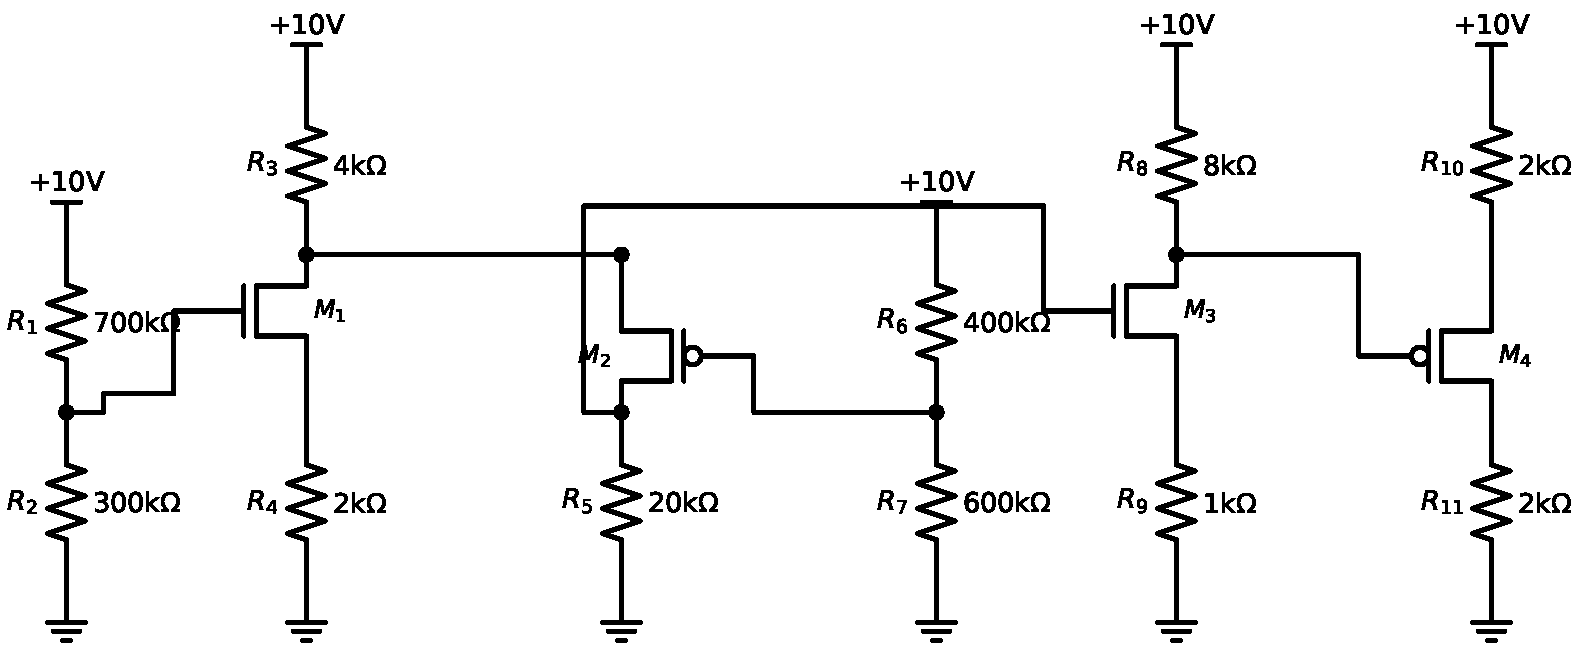
\includegraphics[width=0.9\linewidth,height=6cm,keepaspectratio]{p18_circuit}\end{center}
\solstep{1}{Assumptions}Assume every transistor is active (saturation, tool T1). No current flows into any gate, so gate voltages come from the resistor networks alone.
\solstep{2}{Walk through the circuit}\begin{enumerate}[leftmargin=*,itemsep=3pt]
\item No current flows into a gate ($I_G = 0$), so $V_{G1}$ is set by the divider $R_{1}$--$R_{2}$:\[V_{G1} = 0 + (10 - 0)\frac{300\,\mathrm{k}}{700\,\mathrm{k} + 300\,\mathrm{k}} = 3\,\mathrm{V}\]
\item No current flows into a gate ($I_G = 0$), so $V_{G2}$ is set by the divider $R_{6}$--$R_{7}$:\[V_{G2} = 0 + (10 - 0)\frac{600\,\mathrm{k}}{400\,\mathrm{k} + 600\,\mathrm{k}} = 6\,\mathrm{V}\]
\item KVL from the gate of $M_{1}$ through $V_{GS1}$ and $R_{4}$ ($I_G = 0$, $M_{1}$ assumed active):\[V_{G1} - 0 = 3 = V_{GS1} + R_{4}I_{D1}\]\[I_{D1} = \frac{3 - V_{GS1}}{2\,\mathrm{k}} = \frac{1.1\,\mathrm{m}}{2}(V_{GS1} - 1.4)^2\]\[1.1V_{GS1}^2 - 2.08V_{GS1} - 0.844 = 0 \;\Rightarrow\; V_{GS1} = -0.3434\ \text{or}\ 2.234\,\mathrm{V}\]The root $-0.343$\,V is below $|V_t| = 1.4$\,V (the transistor would be off), so $V_{GS1} = 2.234$\,V. Then $I_{D1} = 383\,\mu \mathrm{A}$ and $V_{S1} = V_{G1} - V_{GS1} = 0.766\,\mathrm{V}$.
\item KVL from the gate of $M_{2}$ through $V_{SG2}$ and $R_{3}$ ($I_G = 0$, $M_{2}$ assumed active):\[10 - V_{G2} = 4 = V_{SG2} + R_{3}(I_{D2} + I_{D1})\]\[I_{D2} = \frac{4 - 4\,\mathrm{k}\times383\,\mu \mathrm{A} - V_{SG2}}{4\,\mathrm{k}} = \frac{850\,\mu }{2}(V_{SG2} - 1.3)^2\]\[1.7V_{SG2}^2 - 3.42V_{SG2} + 0.4044 = 0 \;\Rightarrow\; V_{SG2} = 0.1261\ \text{or}\ 1.886\,\mathrm{V}\]The root $0.126$\,V is below $|V_t| = 1.3$\,V (the transistor would be off), so $V_{SG2} = 1.886$\,V. Then $I_{D2} = 146\,\mu \mathrm{A}$ and $V_{D1} = V_{G2} + V_{SG2} = 7.89\,\mathrm{V}$.
\item $I_{D2} = 146\,\mu \mathrm{A}$ flows through $R_{5}$ to $0$: $V_{D2} = 0 + R_{5}I_{D2} = 0 + 20\,\mathrm{k}\times146\,\mu \mathrm{A} = 2.92\,\mathrm{V}$.
\item KVL from the gate of $M_{3}$ through $V_{GS3}$ and $R_{9}$ ($I_G = 0$, $M_{3}$ assumed active):\[V_{D2} - 0 = 2.915 = V_{GS3} + R_{9}I_{D3}\]\[I_{D3} = \frac{2.915 - V_{GS3}}{1\,\mathrm{k}} = \frac{1.1\,\mathrm{m}}{2}(V_{GS3} - 1.4)^2\]\[0.55V_{GS3}^2 - 0.54V_{GS3} - 1.837 = 0 \;\Rightarrow\; V_{GS3} = -1.401\ \text{or}\ 2.383\,\mathrm{V}\]The root $-1.4$\,V is below $|V_t| = 1.4$\,V (the transistor would be off), so $V_{GS3} = 2.383$\,V. Then $I_{D3} = 532\,\mu \mathrm{A}$ and $V_{S3} = V_{D2} - V_{GS3} = 0.532\,\mathrm{V}$.
\item $I_{D3}$ flows from $10$ through $R_{8}$: $V_{D3} = 10 - R_{8}I_{D3} = 10 - 8\,\mathrm{k}\times532\,\mu \mathrm{A} = 5.75\,\mathrm{V}$.
\item KVL from the gate of $M_{4}$ through $V_{SG4}$ and $R_{10}$ ($I_G = 0$, $M_{4}$ assumed active):\[10 - V_{D3} = 4.254 = V_{SG4} + R_{10}I_{D4}\]\[I_{D4} = \frac{4.254 - V_{SG4}}{2\,\mathrm{k}} = \frac{850\,\mu }{2}(V_{SG4} - 1.3)^2\]\[0.85V_{SG4}^2 - 1.21V_{SG4} - 2.818 = 0 \;\Rightarrow\; V_{SG4} = -1.243\ \text{or}\ 2.667\,\mathrm{V}\]The root $-1.24$\,V is below $|V_t| = 1.3$\,V (the transistor would be off), so $V_{SG4} = 2.667$\,V. Then $I_{D4} = 794\,\mu \mathrm{A}$ and $V_{S4} = V_{D3} + V_{SG4} = 8.41\,\mathrm{V}$.
\item $I_{D4} = 794\,\mu \mathrm{A}$ flows through $R_{11}$ to $0$: $V_{D4} = 0 + R_{11}I_{D4} = 0 + 2\,\mathrm{k}\times794\,\mu \mathrm{A} = 1.59\,\mathrm{V}$.
\end{enumerate}

\solstep{3}{Verify the operating modes}\begin{itemize}[leftmargin=*,itemsep=2pt]
\item $V_{DS1} = V_{D1} - V_{S1} = 7.886 - 0.7657 = 7.12\,\mathrm{V}$ $\ge V_{ov1} = 0.834$\,V $\Rightarrow$ $M_{1}$ is active \checkmark
\item $V_{SD2} = V_{D1} - V_{D2} = 7.886 - 2.915 = 4.97\,\mathrm{V}$ $\ge V_{ov2} = 0.586$\,V $\Rightarrow$ $M_{2}$ is active \checkmark
\item $V_{DS3} = V_{D3} - V_{S3} = 5.746 - 0.5318 = 5.21\,\mathrm{V}$ $\ge V_{ov3} = 0.983$\,V $\Rightarrow$ $M_{3}$ is active \checkmark
\item $V_{SD4} = V_{S4} - V_{D4} = 8.412 - 1.588 = 6.82\,\mathrm{V}$ $\ge V_{ov4} = 1.37$\,V $\Rightarrow$ $M_{4}$ is active \checkmark
\end{itemize}
Unlike the BJT, nothing was neglected here ($I_G = 0$ exactly), so these results are exact for the square-law model: a full nodal solve of the circuit gives the same currents.
\begin{ansbox}
$I_{D1} = 383\,\mu \mathrm{A}$,\quad $I_{D2} = 146\,\mu \mathrm{A}$,\quad $I_{D3} = 532\,\mu \mathrm{A}$,\quad $I_{D4} = 794\,\mu \mathrm{A}$\\[2pt] all transistors active.
\end{ansbox}

\end{document}
